% Options for packages loaded elsewhere
\PassOptionsToPackage{unicode}{hyperref}
\PassOptionsToPackage{hyphens}{url}
\PassOptionsToPackage{dvipsnames,svgnames,x11names}{xcolor}
%
\documentclass[
]{article}
\usepackage{amsmath,amssymb}
\usepackage{iftex}
\ifPDFTeX
  \usepackage[T1]{fontenc}
  \usepackage[utf8]{inputenc}
  \usepackage{textcomp} % provide euro and other symbols
\else % if luatex or xetex
  \usepackage{unicode-math} % this also loads fontspec
  \defaultfontfeatures{Scale=MatchLowercase}
  \defaultfontfeatures[\rmfamily]{Ligatures=TeX,Scale=1}
\fi
\usepackage{lmodern}
\ifPDFTeX\else
  % xetex/luatex font selection
\fi
% Use upquote if available, for straight quotes in verbatim environments
\IfFileExists{upquote.sty}{\usepackage{upquote}}{}
\IfFileExists{microtype.sty}{% use microtype if available
  \usepackage[]{microtype}
  \UseMicrotypeSet[protrusion]{basicmath} % disable protrusion for tt fonts
}{}
\makeatletter
\@ifundefined{KOMAClassName}{% if non-KOMA class
  \IfFileExists{parskip.sty}{%
    \usepackage{parskip}
  }{% else
    \setlength{\parindent}{0pt}
    \setlength{\parskip}{6pt plus 2pt minus 1pt}}
}{% if KOMA class
  \KOMAoptions{parskip=half}}
\makeatother
\usepackage{xcolor}
\usepackage[a4paper,margin=1in]{geometry}
\usepackage{graphicx}
\makeatletter
\def\maxwidth{\ifdim\Gin@nat@width>\linewidth\linewidth\else\Gin@nat@width\fi}
\def\maxheight{\ifdim\Gin@nat@height>\textheight\textheight\else\Gin@nat@height\fi}
\makeatother
% Scale images if necessary, so that they will not overflow the page
% margins by default, and it is still possible to overwrite the defaults
% using explicit options in \includegraphics[width, height, ...]{}
\setkeys{Gin}{width=\maxwidth,height=\maxheight,keepaspectratio}
% Set default figure placement to htbp
\makeatletter
\def\fps@figure{htbp}
\makeatother
\setlength{\emergencystretch}{3em} % prevent overfull lines
\providecommand{\tightlist}{%
  \setlength{\itemsep}{0pt}\setlength{\parskip}{0pt}}
\setcounter{secnumdepth}{-\maxdimen} % remove section numbering
\usepackage{xcolor}
\usepackage{graphicx}
\usepackage{hyperref}
\usepackage{eso-pic}
\usepackage{draftwatermark}
\SetWatermarkText{DRAFT}
\SetWatermarkScale{1}
\SetWatermarkAngle{45}
\SetWatermarkColor{gray!10}
\usepackage{etoolbox}
\AtBeginEnvironment{Shaded}{\small}
\usepackage{booktabs}
\usepackage{longtable}
\usepackage{array}
\usepackage{multirow}
\usepackage{wrapfig}
\usepackage{float}
\usepackage{colortbl}
\usepackage{pdflscape}
\usepackage{tabularx}
\usepackage{xltabular}
\usepackage{threeparttable}
\usepackage{threeparttablex}
\usepackage[normalem]{ulem}
\usepackage{makecell}
\usepackage{xcolor}
\ifLuaTeX
  \usepackage{selnolig}  % disable illegal ligatures
\fi
\usepackage{bookmark}
\IfFileExists{xurl.sty}{\usepackage{xurl}}{} % add URL line breaks if available
\urlstyle{same}
\hypersetup{
  colorlinks=true,
  linkcolor={black},
  filecolor={Maroon},
  citecolor={Blue},
  urlcolor={blue},
  pdfcreator={LaTeX via pandoc}}

\author{}
\date{\vspace{-2.5em}}

\begin{document}

\null
\thispagestyle{empty}
\clearpage

\begin{center}
\vspace*{0.18\textheight}

{\Huge\bfseries 1 Formula\par}
\vspace{1em}
{\Large A Mathematical Analysis to Identify the Top Formula 1 Driver in History\par}
\vspace{2em}
Jean-Marie Roy\par
2026-11-15

\vspace*{\fill}

\includegraphics[width=0.2\textwidth]{/home/runner/work/Formula-1/Formula-1/images/report/flag.png}
\vspace*{1em}
\end{center}

\newpage

\tableofcontents

\newpage

\section{1. Introduction}\label{introduction}

When posed the question, ``Who is or was the best Formula 1 driver of
all time?'' an AI agent will likely first mention \textbf{Lewis
Hamilton}, followed by \textbf{Michael Schumacher}, based primarily on
their respective world championship titles. If asked for a list of top
drivers, it might also include \textbf{Juan Manuel Fangio},
\textbf{Alain Prost}, \textbf{Max Verstappen}, and \textbf{Sebastian
Vettel}, arranged alphabetically. \textbf{Fangio} stands out with five
championships, while the others each have four.

Interestingly, many fans regard \textbf{Ayrton Senna}, with his three
titles, as a superior driver compared to \textbf{Alain Prost}, despite
the latter's four championships. This raises the question: how
significant are titles in evaluating a driver's greatness? Should we
consider alternative criteria for determining who truly excels?

If we delve deeper, \textbf{Juan Manuel Fangio} won five titles in the
1950s, during the formative years of the Formula 1 World Championship.
His legacy is so profound that his name has become synonymous with
exceptional driving. In French-speaking regions, the phrase ``driving
like Fangio'' denotes flawless driving. A notable reference appears in
\emph{The Adventures of Tintin: The Calculus Affair} {[}1{]}, where a
character remarks, ``This must be Fangio at the wheel'' as a car
skillfully avoids a net, reflecting Fangio's prowess during the height
of his career. (In the English edition, it is translated as \emph{``They
must have a Jack Brabham at the wheel!''})

\begin{figure}

{\centering 
\includegraphics[width=0.7\linewidth]{../images/report/tintin} 

}

\caption{\textit{"This must be Fangio at the wheel!"}}\label{fig:unnamed-chunk-9}
\end{figure}

Complicating matters further, the rules of Formula 1 have evolved
significantly over the years. The number of races has increased (from
seven during Fangio's era to 22 today), and the points system has
undergone various changes. For instance, the winner received 8 points
until \textbf{1960}, then 9 points until \textbf{1990}, followed by 10
points until \textbf{2009}, and has been set at 25 points since
\textbf{2010}. Additionally, until \textbf{1990}, only the best results
counted towards the championship, which allowed Senna to secure the
title in \textbf{1990} against Prost, despite the latter having more
points overall; under modern rules, Prost would have been awarded the
title instead.

Ultimately, it is evident that even the most skilled drivers depend
significantly on their cars' performance. Both Alain Prost in
\textbf{1991} and Lewis Hamilton in \textbf{2025} encountered
substantial difficulties while driving for Ferrari, so much so that
Prost was dismissed from his team after comparing his car to a
``truck.'' This raises an important question: to what extent is a world
title attributable to the car, and how much is a reflection of the
driver's ability?

\newpage

\section{2. Dataset}\label{dataset}

\subsection{2.1 Source}\label{source}

The data used throughout this study comes from \textbf{Jolpica F1}
{[}2{]}, an open-source (Apache 2.0) Formula 1 API maintained by a group
of volunteers. Jolpica was created as the successor to the widely used
Ergast API, which was deprecated at the end of the 2024 season, and
provides the same type of historical data (drivers, teams, sessions,
results, standings, lap times and pit stops) through a redesigned
database schema. According to its maintainers, this new schema is
intended to better accommodate changing rule sets, reduce duplicated
information and allow the storage of additional F1-related data.

As Jolpica is an independent open-source project, its internals ---
scraping process, data validation and correction policies --- are the
responsibility of its maintainers and are outside the scope of this
work. We therefore treat Jolpica as the \emph{system of record} for
historical Formula 1 data and restrict ourselves to documenting how the
data is ingested, transformed and audited on our side. A full
description of the tables can be found in the project's database
documentation {[}3{]}.

It should be noted that Jolpica publishes its database dump with a delay
of approximately two weeks: more recent data is only available through a
paid tier. Since this study analyses historical data up to the end of
the previous season --- deliberately excluding the ongoing season ---
the free release is entirely sufficient, and the delayed publication has
no impact on the completeness of the dataset used here.

\subsection{2.2 Pipeline}\label{pipeline}

The ingestion, transformation and publication of the data is fully
automated in an ELT pipeline published on GitHub {[}4{]}, orchestrated
with \textbf{GitHub Actions} and scheduled to run \textbf{weekly} (with
manual triggering also possible). The pipeline extracts the raw data
from Jolpica and produces two outputs: a normalised SQLite database used
for validation and transformation, and a mirror of the raw tables in
Databricks used for interactive analysis.

The pipeline performs the following steps:

\begin{enumerate}
\def\labelenumi{\arabic{enumi}.}
\tightlist
\item
  \textbf{Extract} --- the full Jolpica database dump (18 CSV files, one
  per table, \textasciitilde40 MB compressed) is downloaded from the
  Jolpica data endpoint. A freshness check skips the download if the
  data is less than 7 days old, and the original Ergast/Jolpica table
  schemas are preserved.
\item
  \textbf{Load} --- the raw CSVs are normalised into a \textbf{star
  schema SQLite} database (\texttt{jolpica.db}), with foreign key
  validation guaranteeing referential integrity. This database
  (\textasciitilde900K rows covering every F1 race since 1950) acts as a
  portable, version-controlled snapshot of the raw data, fully
  independent from any cloud service.
\item
  \textbf{Transform} --- running in parallel with the publication step,
  the transformation job reshapes the raw schema into an analytics
  schema (\texttt{formula1.db}), adds derived fields (driver age,
  cumulative points, country flags), and applies \textbf{dbt} models and
  tests on top.
\item
  \textbf{Publish to Databricks} --- each raw SQLite table is exported
  to Parquet, staged in a Unity Catalog volume, and loaded into
  \textbf{Delta tables} in Databricks via \texttt{COPY\ INTO}, with
  automatic type widening and row-count verification against the source.
  This gives a queryable copy of the raw dataset for exploratory
  analysis without needing to download the SQLite file.
\end{enumerate}

\newpage

The two branches of the pipeline are intentionally decoupled: a
Databricks outage cannot block the local SQLite build and release.

\begin{figure}

{\centering 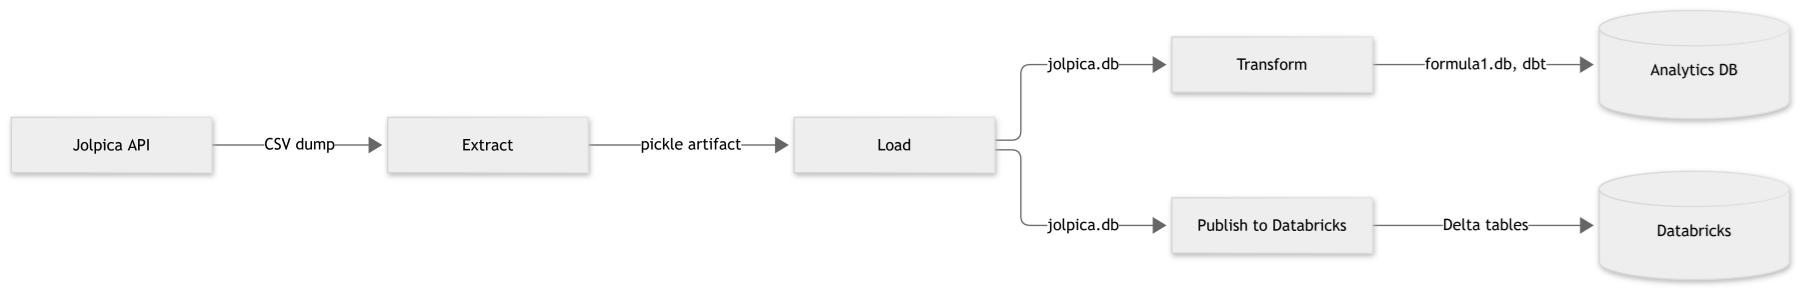
\includegraphics[width=1\linewidth]{../images/report/pipeline} 

}

\caption{Pipeline architecture: Jolpica → SQLite → dbt / Databricks}\label{fig:unnamed-chunk-13}
\end{figure}

Two design decisions are worth highlighting, as they affect the
reproducibility of the analysis:

\begin{itemize}
\tightlist
\item
  \textbf{Full reload instead of incremental processing.} With roughly
  900K rows, reloading the entire dataset at each run is cheap, and ---
  more importantly --- safe: F1 stewards occasionally issue
  disqualifications or points adjustments \emph{after} races, so
  append-only logic would silently miss retroactive corrections. This is
  particularly relevant for the historical quirks discussed in Section
  2.4.
\item
  \textbf{Release strategy.} The database is distributed via GitHub
  Releases under a mutable \texttt{data-latest} tag, overwritten at each
  run. Versioned immutable releases (\texttt{data-YYYYMMDD}) are a
  planned improvement; for this study, the dataset snapshot used for the
  analysis is documented together with the results to ensure
  reproducibility.
\end{itemize}

The pipeline consumes a single input: the Jolpica database dump,
delivered as a ZIP archive of 18 CSV files, one per table. The table
below lists these input files as recorded in the database inventory;
each file corresponds one-to-one with a table described in Section 2.3.

\begin{table}[!h]
\centering\begingroup\fontsize{9}{11}\selectfont

\begin{tabular}[t]{llllll}
\toprule
 & Files &  &  &  & \\
\midrule
\includegraphics[width=0.5cm]{/home/runner/work/Formula-1/Formula-1/images/report/file-csv.png} & base\_team.csv & \includegraphics[width=0.5cm]{/home/runner/work/Formula-1/Formula-1/images/report/file-csv.png} & lap.csv & \includegraphics[width=0.5cm]{/home/runner/work/Formula-1/Formula-1/images/report/file-csv.png} & season.csv\\
\includegraphics[width=0.5cm]{/home/runner/work/Formula-1/Formula-1/images/report/file-csv.png} & championship\_adjustment.csv & \includegraphics[width=0.5cm]{/home/runner/work/Formula-1/Formula-1/images/report/file-csv.png} & penalty.csv & \includegraphics[width=0.5cm]{/home/runner/work/Formula-1/Formula-1/images/report/file-csv.png} & session.csv\\
\includegraphics[width=0.5cm]{/home/runner/work/Formula-1/Formula-1/images/report/file-csv.png} & championship\_system.csv & \includegraphics[width=0.5cm]{/home/runner/work/Formula-1/Formula-1/images/report/file-csv.png} & pit\_stop.csv & \includegraphics[width=0.5cm]{/home/runner/work/Formula-1/Formula-1/images/report/file-csv.png} & session\_entry.csv\\
\includegraphics[width=0.5cm]{/home/runner/work/Formula-1/Formula-1/images/report/file-csv.png} & circuit.csv & \includegraphics[width=0.5cm]{/home/runner/work/Formula-1/Formula-1/images/report/file-csv.png} & points\_system.csv & \includegraphics[width=0.5cm]{/home/runner/work/Formula-1/Formula-1/images/report/file-csv.png} & team.csv\\
\includegraphics[width=0.5cm]{/home/runner/work/Formula-1/Formula-1/images/report/file-csv.png} & driver.csv & \includegraphics[width=0.5cm]{/home/runner/work/Formula-1/Formula-1/images/report/file-csv.png} & round.csv & \includegraphics[width=0.5cm]{/home/runner/work/Formula-1/Formula-1/images/report/file-csv.png} & team\_championship.csv\\
\includegraphics[width=0.5cm]{/home/runner/work/Formula-1/Formula-1/images/report/file-csv.png} & driver\_championship.csv & \includegraphics[width=0.5cm]{/home/runner/work/Formula-1/Formula-1/images/report/file-csv.png} & roundentry.csv & \includegraphics[width=0.5cm]{/home/runner/work/Formula-1/Formula-1/images/report/file-csv.png} & team\_driver.csv\\
\bottomrule
\end{tabular}
\endgroup{}
\end{table}

\newpage

\subsection{2.3 Tables}\label{tables}

\subsubsection{2.3.0 Overview}\label{overview}

The Jolpica export consists of \textbf{18 tables} covering seasons,
rounds, circuits, sessions, results, teams, championships, scoring
systems, lap times, pit stops and staging tables. Note that the schema
intentionally differs from Ergast's: Jolpica splits the old monolithic
races/results concepts into fine-grained round, session and
session\_entry tables, which allows a modern race weekend (practice,
qualifying, sprint, race) to be modelled explicitly.

\subsubsection{2.3.1 Core Season \& Race
Structure}\label{core-season-race-structure}

The three tables below form the backbone of the temporal dimension: they
identify each season, each Grand Prix, and each physical circuit.

\begin{table}[!h]
\centering\begingroup\fontsize{9}{11}\selectfont

\begin{tabular}[t]{>{\raggedright\arraybackslash}p{4.5cm}>{\raggedright\arraybackslash}p{1.5cm}>{\raggedright\arraybackslash}p{9cm}}
\toprule
Table & Rows & Purpose\\
\midrule
\texttt{season} & 77 & Master record of every F1 season (1950-present). Contains year, championship system reference, and Wikipedia link. Primary time dimension for all temporal queries.\\
\texttt{round} & 1,173 & Individual Grands Prix within seasons. Links to season and circuit, includes race number, official name, date, and Wikipedia reference. Represents the traditional race event concept.\\
\texttt{circuit} & 78 & Physical racetracks. Stores track metadata including location data and Wikipedia URL. Rarely changes over time - a dimensional lookup table.\\
\bottomrule
\end{tabular}
\endgroup{}
\end{table}

\subsubsection{2.3.2 Session-Level Detail}\label{session-level-detail}

Modern Formula 1 weekends comprise multiple timed sessions (practice,
qualifying, sprint, race). Jolpica models this explicitly with two
tables:

\begin{table}[!h]
\centering\begingroup\fontsize{9}{11}\selectfont

\begin{tabular}[t]{>{\raggedright\arraybackslash}p{4.5cm}>{\raggedright\arraybackslash}p{1.5cm}>{\raggedright\arraybackslash}p{9cm}}
\toprule
Table & Rows & Purpose\\
\midrule
\texttt{session} & 5,130 & Granular timing sessions (Race, Qualifying, Sprint, Practice). Modern F1 structure where a round may have multiple sessions. Includes scheduled laps, timezone, and cancellation flags.\\
\texttt{session\_entry} & 52,049 & Driver results per session. Contains grid position, finishing position, points scored, laps completed, time/difference, status codes, and classification eligibility. Most frequently queried results table.\\
\bottomrule
\end{tabular}
\endgroup{}
\end{table}

\newpage

\subsubsection{2.3.3 Driver \& Constructor
Records}\label{driver-constructor-records}

Drivers and constructors are tracked both as profiles and as historical
pairings, alongside the legacy entry mechanism used before session-level
granularity:

\begin{table}[!h]
\centering\begingroup\fontsize{9}{11}\selectfont

\begin{tabular}[t]{>{\raggedright\arraybackslash}p{4.5cm}>{\raggedright\arraybackslash}p{1.5cm}>{\raggedright\arraybackslash}p{9cm}}
\toprule
Table & Rows & Purpose\\
\midrule
\texttt{driver} & 884 & Driver profiles: names, nationality, date of birth and country. Core dimension for any driver-level aggregation; driver age at race date is derived from it during transformation.\\
\texttt{team} & 214 & All constructor entries in history. Note: constructors evolve or rebrand - this tracks distinct legal entities, not just Ferrari/Mercedes/Red Bull brand names.\\
\texttt{team\_driver} & 3,633 & Historical pairings of which driver drove for which team. Junction table linking drivers and teams, with validity periods implied by related records.\\
\texttt{roundentry} & 27,740 & Which team-driver combination entered which round (before session granularity). Contains car number assignment. Legacy linkage from older schema design.\\
\bottomrule
\end{tabular}
\endgroup{}
\end{table}

\subsubsection{2.3.4 Championship
Standings}\label{championship-standings}

Both championships are tracked cumulatively after every round, enabling
trajectory analysis over the course of a season:

\begin{table}[!h]
\centering\begingroup\fontsize{9}{11}\selectfont

\begin{tabular}[t]{>{\raggedright\arraybackslash}p{4.5cm}>{\raggedright\arraybackslash}p{1.5cm}>{\raggedright\arraybackslash}p{9cm}}
\toprule
Table & Rows & Purpose\\
\midrule
\texttt{driver\_championship} & 36,869 & Cumulative driver standings across the season. Tracks points accumulation after each round - enabling analysis of championship trajectories, comebacks, and mathematical elimination dates.\\
\texttt{team\_championship} & 14,579 & Equivalent constructor standings. Mirrors the driver championship table structure but for teams. Critical for analysing constructor battles and historic dominance patterns.\\
\bottomrule
\end{tabular}
\endgroup{}
\end{table}

\subsubsection{2.3.5 Scoring Systems}\label{scoring-systems}

Point allocation has changed repeatedly across F1 history. Three tables
document the rules governing how results translate into points:

\begin{table}[!h]
\centering\begingroup\fontsize{9}{11}\selectfont

\begin{tabular}[t]{>{\raggedright\arraybackslash}p{4.5cm}>{\raggedright\arraybackslash}p{1.5cm}>{\raggedright\arraybackslash}p{9cm}}
\toprule
Table & Rows & Purpose\\
\midrule
\texttt{points\_system} & 24 & Historical point-allocation rules. Each row defines a unique scoring scheme used during a period, explaining why different eras award points differently.\\
\texttt{championship\_system} & 11 & Broader championship format definitions. May encompass tiebreaker rules, sprint weekend variants, or multi-season aggregations.\\
\texttt{championship\_adjustment} & 3 & Special corrections to historical standings. Likely captures retroactive disqualifications, title rescissions, or corrections to original records.\\
\bottomrule
\end{tabular}
\endgroup{}
\end{table}

\newpage

\subsubsection{2.3.6 Performance Metrics}\label{performance-metrics}

Two high-cardinality tables capture on-track performance:

\begin{table}[!h]
\centering\begingroup\fontsize{9}{11}\selectfont

\begin{tabular}[t]{>{\raggedright\arraybackslash}p{4.5cm}>{\raggedright\arraybackslash}p{1.5cm}>{\raggedright\arraybackslash}p{9cm}}
\toprule
Table & Rows & Purpose\\
\midrule
\texttt{lap} & 741,763 & Per-lap timing data. The highest-cardinality table, containing individual lap times for every driver in every race session. Essential for pace analysis, fastest-lap identification, and tyre-strategy modelling.\\
\texttt{pit\_stop} & 13,087 & Pit-stop events, including duration and timing within a race, and potentially crew performance data. Critical for race-strategy analysis and comparing pit-crew performance.\\
\bottomrule
\end{tabular}
\endgroup{}
\end{table}

\subsubsection{2.3.7 Staging Tables (Not Used in
Analysis)}\label{staging-tables-not-used-in-analysis}

Two tables exist as empty staging structures with no analytical value:

\begin{table}[!h]
\centering\begingroup\fontsize{9}{11}\selectfont

\begin{tabular}[t]{>{\raggedright\arraybackslash}p{4.5cm}>{\raggedright\arraybackslash}p{1.5cm}>{\raggedright\arraybackslash}p{9cm}}
\toprule
Table & Rows & Purpose\\
\midrule
\texttt{base\_team} & 0 & Empty staging table - likely intended for ETL operations or future use. Currently contains no data.\\
\texttt{penalty} & 0 & Intended for driver or constructor penalties but currently empty. It may be populated by future pipeline updates or used only when infractions occur.\\
\bottomrule
\end{tabular}
\endgroup{}
\end{table}

\newpage

\subsection{2.4 Quick Analysis}\label{quick-analysis}

\subsubsection{2.4.1 A First Look at the Raw
Tables}\label{a-first-look-at-the-raw-tables}

Before describing the issues hidden in the data, it is worth looking at
the tables themselves. The extracts below show the first rows of two
tables --- \texttt{season}, one of the smallest tables in the schema,
and \texttt{pit\_stop}, a fact table --- chosen so that all their
columns fit on the page.

First, the \texttt{season} table --- with only a handful of rows and
columns, it defines the championship calendar:

\begin{table}[!h]
\centering\begingroup\fontsize{8}{10}\selectfont

\resizebox{\ifdim\width>\linewidth\linewidth\else\width\fi}{!}{
\begin{tabular}[t]{rrlrl}
\toprule
id & year & api\_id & championship\_system\_id & wikipedia\\
\midrule
1 & 1950 & season\_oPqQEC4b & 1 & https://en.wikipedia.org/wiki/1950\_Formula\_One\_season\\
2 & 1951 & season\_nH07GTj5 & 1 & https://en.wikipedia.org/wiki/1951\_Formula\_One\_season\\
3 & 1952 & season\_AkHDeRX4 & 1 & https://en.wikipedia.org/wiki/1952\_Formula\_One\_season\\
4 & 1953 & season\_E63rvZZO & 1 & https://en.wikipedia.org/wiki/1953\_Formula\_One\_season\\
5 & 1954 & season\_B36NWfA1 & 2 & https://en.wikipedia.org/wiki/1954\_Formula\_One\_season\\
\bottomrule
\end{tabular}}
\endgroup{}
\end{table}

The extract below shows the first rows of the \texttt{pit\_stop} table:

\begin{table}[!h]
\centering\begingroup\fontsize{8}{10}\selectfont

\resizebox{\ifdim\width>\linewidth\linewidth\else\width\fi}{!}{
\begin{tabular}[t]{rrrrlll}
\toprule
id & session\_entry\_id & lap\_id & number & duration & local\_timestamp & api\_id\\
\midrule
1 & 27696 & 275638 & 2 & 00:00:24.036 & 17:59:17 & pitstop\_IYavKg2C\\
2 & 27696 & 275672 & 1 & 00:00:22.603 & 17:25:17 & pitstop\_XDzyA9tn\\
3 & 27700 & 275742 & 1 & 00:00:23.227 & 17:28:24 & pitstop\_c0OV7PJY\\
4 & 27700 & 275746 & 2 & 00:00:23.199 & 17:59:29 & pitstop\_SFBiesKg\\
5 & 27704 & 275769 & 1 & 00:00:24.535 & 17:28:39 & pitstop\_ZS3hcaW8\\
\bottomrule
\end{tabular}}
\endgroup{}
\end{table}

\subsubsection{\texorpdfstring{2.4.2 The \texttt{api\_id}
Column}{2.4.2 The api\_id Column}}\label{the-api_id-column}

The two extracts above reveal a common pattern: every table begins with
an \texttt{api\_id} column. This identifier is present in \textbf{all 18
tables} of the export --- inspecting the remaining tables (not
reproduced here) shows exactly the same structure. It mirrors the
primary key exposed by the Jolpica API and is therefore
\emph{application specific}: it identifies records within Jolpica's own
infrastructure (and its Ergast-compatible endpoints) rather than
describing anything about the racing data itself.

Since it carries no analytical meaning, duplicates the information
already present in the pipeline's own keys, and wastes width in every
table, \textbf{these columns will be dropped from all tables during the
dbt transformation step}; the details are covered in Chapter 3.

Dropping the columns from the analytical tables does not mean discarding
the information permanently. Should the values ever prove useful again
--- for example, for tracing records back to Jolpica's endpoints or for
debugging the extraction process --- they could be preserved in
dedicated, application-level lookup tables, kept strictly separate from
the F1 data tables described above.

\newpage

\subsubsection{2.4.3 Winner Uniqueness}\label{winner-uniqueness}

The most basic integrity expectation for a results table is that each
race has exactly one winner. This expectation is, however, merely an
assumption made by the analyst --- the raw export is never accompanied
by a formal definition of what constitutes a unique race winner --- and
is therefore worth verifying explicitly.

Working directly from the Jolpica \texttt{results} table, a simple count
of drivers classified in first position per race confirms two things.
First, no race in the dataset lacks a winner altogether; second, several
races list \textbf{more than one} driver in first position:

\begin{table}[!h]
\centering\begingroup\fontsize{8}{10}\selectfont

\resizebox{\ifdim\width>\linewidth\linewidth\else\width\fi}{!}{
\begin{tabular}[t]{rr}
\toprule
id & n\_winners\\
\midrule
31 & 2\\
145 & 2\\
181 & 2\\
\bottomrule
\end{tabular}}
\endgroup{}
\end{table}

To identify the affected races, the races listing more than one winner
are then joined with the \texttt{races} and \texttt{drivers} tables ---
the joins serve purely to attach human-readable context, not to derive
the counts:

\begin{table}[!h]
\centering\begingroup\fontsize{8}{10}\selectfont

\resizebox{\ifdim\width>\linewidth\linewidth\else\width\fi}{!}{
\begin{tabular}[t]{rlr}
\toprule
year & circuit & n\_winners\\
\midrule
1951 & French Grand Prix & 2\\
1956 & Argentine Grand Prix & 2\\
1957 & British Grand Prix & 2\\
\bottomrule
\end{tabular}}
\endgroup{}
\end{table}

At first glance this looks like a data-quality defect, but it turns out
to be a historically faithful representation of the sport's earliest
era, as the next section explains.

\subsubsection{2.4.4 Shared Drives in the Early
Years}\label{shared-drives-in-the-early-years}

The multiple-winner phenomenon observed above is not an error in the
export but a consequence of a practice that was accepted in Formula
One's formative years: \textbf{car sharing}. In the early seasons, teams
frequently entered smaller fields than the grid size, and a single car
could be driven by several drivers over the course of one race --- one
driver starting the race and another taking over later, in the manner of
an endurance relay.

Under the regulations of the time, all drivers who took the wheel were
credited with the race result achieved by that car. Consequently, when a
shared car finished first, the results table records several drivers
sharing the win --- exactly the pattern surfaced by the aggregation in
Section 2.4.3. The same convention extends beyond victories: position
assignments, classifications, and championship points accrued by such
cars were likewise divided among the participating drivers.

From a data-modelling perspective, this means the natural key of the
results table is not (race, position) alone, since a single finishing
position can legitimately be occupied by multiple driver rows. Any
transformation or analysis step must therefore account for this
historical peculiarity rather than treating duplicate positions as
anomalies to be corrected.

\newpage

\subsubsection{2.4.5 Fractional Point
Values}\label{fractional-point-values}

The shared-drive practice of Section 2.4.4 leaves an arithmetic
fingerprint in the \texttt{points} column --- but it is not the only
source of non-integer point values. Up to this point the integrity
checks have concerned the \emph{structural} attributes of the export ---
keys, positions, flags; the \texttt{points} column itself has not been
inspected yet, even though it encodes the accumulated effect of every
historical scoring quirk. Championship points are expected to be whole
numbers --- or, at worst, halves --- so a natural first check is to ask
which values violate this expectation. The query below surveys every
non-integer value appearing anywhere in the results and counts how many
rows carry each fractional part:

\begin{table}[!h]
\centering\begingroup\fontsize{8}{10}\selectfont

\resizebox{\ifdim\width>\linewidth\linewidth\else\width\fi}{!}{
\begin{tabular}[t]{rr}
\toprule
fractional\_part & n\_rows\\
\midrule
0.50 & 35\\
0.14 & 7\\
0.33 & 3\\
\bottomrule
\end{tabular}}
\endgroup{}
\end{table}

The distribution is remarkably clean: the overwhelming majority of
fractional rows carry an exact half, while only two much finer fractions
appear at all. Several distinct, well-documented mechanisms can produce
exact halves, and they are worth enumerating before attempting to
attribute individual rows:

\begin{itemize}
\tightlist
\item
  \textbf{Abandoned races.} When a Grand Prix was halted before the full
  distance had been covered --- typically by torrential rain or a
  serious accident, with the race unable to resume --- drivers received
  \textbf{half} of the points attached to their finishing position. A
  driver classified fourth in such a race, a placement worth 3 points
  under the scoring systems that governed the sport for its first four
  decades, was consequently credited with 1.5 points. Rain-shortened
  editions appear irregularly across the entire history of the
  championship.
\item
  \textbf{Shared drives.} Whenever \emph{two} drivers shared one car
  that finished in a points-paying position, the points attached to that
  place were divided equally between them (Section 2.4.4), and a
  division of an integer by two again yields exactly one half.
\item
  \textbf{Shared fastest-lap points.} Under the early scoring systems,
  the bonus point attached to the fastest lap could be \textbf{split}
  when two drivers recorded an identical fastest time --- each taking
  half of the single point. A driver who finished in a points-paying
  position and co-held the fastest lap thus carries a half appended to
  an otherwise integral total: second place under the 1950--1959 system
  (6 points) plus half the bonus yields 6.5. This is the two-driver case
  of the seven-way split examined in Section 2.4.6.
\end{itemize}

Attributing each individual half to its mechanism is more delicate than
it may seem, and naive heuristics fail quickly: a points value is the
\emph{sum} of position points and a possible bonus share, so either
component may be the halved one, and the mechanisms are not mutually
exclusive --- a shared car in a rain-shortened race is divided twice
over, yielding quarters. Rather than attempting a per-row
classification, the survey above is treated as evidence that all
fractional values fall within a known, historically grounded set of
mechanisms. What \emph{cannot} be explained by any of them are the
values that are neither integers nor exact halves, visible at the tail
of the extract; isolating them pins down only two affected races, which
the next section inspects individually.

\newpage

\subsubsection{2.4.6 Finer Fractions from Shared
Awards}\label{finer-fractions-from-shared-awards}

Values that are neither integers nor exact halves resist the explanation
of Section 2.4.5 and require a closer look. Isolating them from the
unique point values of the \texttt{session\_entry} table yields only two
contaminated races:

\begin{table}[!h]
\centering\begingroup\fontsize{8}{10}\selectfont

\resizebox{\ifdim\width>\linewidth\linewidth\else\width\fi}{!}{
\begin{tabular}[t]{rlllrr}
\toprule
year & circuit & driver & team & position & points\\
\midrule
1954 & British Grand Prix & José Froilán González & Ferrari & 1 & 8.14\\
1954 & British Grand Prix & Mike Hawthorn & Ferrari & 2 & 6.14\\
1954 & British Grand Prix & Onofre Marimón & Maserati & 3 & 4.14\\
1954 & British Grand Prix & Juan Fangio & Mercedes & 4 & 3.14\\
1954 & British Grand Prix & Stirling Moss & Maserati & 16 & 0.14\\
1954 & British Grand Prix & Jean Behra & Gordini & 18 & 0.14\\
1954 & British Grand Prix & Alberto Ascari & Maserati & 24 & 0.14\\
1955 & Argentine Grand Prix & Umberto Maglioli & Ferrari & 3 & 1.33\\
1955 & Argentine Grand Prix & Nino Farina & Ferrari & 3 & 1.33\\
1955 & Argentine Grand Prix & Maurice Trintignant & Ferrari & 3 & 1.33\\
\bottomrule
\end{tabular}}
\endgroup{}
\end{table}

Both races illustrate points being \textbf{divided rather than awarded},
each in its own way. At the 1954 British Grand Prix, every affected
driver carries an identical increment of 1/7 point on top of the points
earned by finishing position --- the fastest-lap bonus point of the
era's scoring system, awarded jointly to seven drivers who set an
identical fastest lap and thus shared its single point seven ways. At
the 1955 Argentine Grand Prix, three drivers sharing one car finished
jointly in third position; the four points attached to that place were
divided equally, each driver recording 4/3 points. Both mechanisms are
consequences of the shared-car and shared-award practices of the period
described in Section 2.4.4, confined to the 1950s --- confirming that
these fractions are faithful historical records rather than pipeline
errors.

\subsubsection{2.4.7 The Absent Fastest
Lap}\label{the-absent-fastest-lap}

Among the shared awards of Section 2.4.6, one subset deserves a final
inspection: the drivers who received 1/7 of the fastest-lap point at the
1954 British Grand Prix. Their fractional increment of
\textasciitilde0.14 makes them easy to isolate, and their rows are
informative --- although a fastest-lap award is recorded in the
\texttt{points} column, the dedicated \texttt{fastest\_lap\_rank} column
remains empty for every one of them:

\begin{table}[!h]
\centering\begingroup\fontsize{8}{10}\selectfont

\resizebox{\ifdim\width>\linewidth\linewidth\else\width\fi}{!}{
\begin{tabular}[t]{rlllrrr}
\toprule
year & circuit & driver & team & position & points & fastest\_lap\_rank\\
\midrule
1954 & British Grand Prix & José Froilán González & Ferrari & 1 & 8.14 & NA\\
1954 & British Grand Prix & Mike Hawthorn & Ferrari & 2 & 6.14 & NA\\
1954 & British Grand Prix & Onofre Marimón & Maserati & 3 & 4.14 & NA\\
1954 & British Grand Prix & Juan Fangio & Mercedes & 4 & 3.14 & NA\\
1954 & British Grand Prix & Stirling Moss & Maserati & 16 & 0.14 & NA\\
1954 & British Grand Prix & Jean Behra & Gordini & 18 & 0.14 & NA\\
1954 & British Grand Prix & Alberto Ascari & Maserati & 24 & 0.14 & NA\\
\bottomrule
\end{tabular}}
\endgroup{}
\end{table}

The seven \texttt{NA} values in the extract are not an accidental
omission of these particular rows, but a coverage boundary of the
source: the dataset contains fastest-lap records only starting from the
1958 season, earlier editions of the championship having no officially
tracked fastest lap. The boundary can be located precisely in the data:

\begin{table}[!h]
\centering\begingroup\fontsize{8}{10}\selectfont

\resizebox{\ifdim\width>\linewidth\linewidth\else\width\fi}{!}{
\begin{tabular}[t]{r}
\toprule
first\_season\_with\_fastest\_lap\\
\midrule
1958\\
\bottomrule
\end{tabular}}
\endgroup{}
\end{table}

The situation is therefore somewhat ironic: the very drivers who
\emph{jointly} set the fastest lap in 1954 cannot be recognised as such
from the \texttt{fastest\_lap\_rank} column. Closing this gap is a
candidate for the transformation work described in Chapter 3:
fastest-lap data for the earlier seasons could be integrated from an
external source as part of the planned modifications, restoring complete
coverage of this statistic across the championship's history.

\subsubsection{2.4.8 Ineligible Drivers Who Scored
Points}\label{ineligible-drivers-who-scored-points}

The last integrity check concerns the consistency between the
eligibility flag and the \texttt{points} column. Every row of the
results carries an \texttt{is\_eligible\_for\_points} indicator, and the
naive expectation is a strict correspondence: drivers flagged as
ineligible should record zero points. The export violates this
expectation exactly once:

\begin{table}[!h]
\centering\begingroup\fontsize{8}{10}\selectfont

\resizebox{\ifdim\width>\linewidth\linewidth\else\width\fi}{!}{
\begin{tabular}[t]{rlllrrlr}
\toprule
year & circuit & driver & team & position & points & detail & laps\_completed\\
\midrule
1956 & Monaco Grand Prix & Juan Fangio & Ferrari & 4 & 1.5 & +1 Lap & 99\\
\bottomrule
\end{tabular}}
\endgroup{}
\end{table}

Consulting the historical record resolves the apparent contradiction,
and it involves the shared-drive practice of Section 2.4.4 twice over.
At the 1956 Monaco Grand Prix, Juan Manuel Fangio drove two cars: he
shared the car number 26, which finished second, with Peter Collins, and
the car number 20, which finished fourth, with Eugenio Castellotti.
Under the regulations of the time, the points of a shared car were
divided among its drivers --- but a driver who had already received
points from one car was \textbf{not entitled to collect points from a
second one}. Fangio therefore took his half of the second-place points
(three of six, shared with Collins), while his would-be share of the
fourth place --- three points divided by two, the 1.5 recorded in the
extract --- went uncollected.

The extract below places this single violating row in its full context
by listing every Ferrari entry of that race:

\begin{table}[!h]
\centering\begingroup\fontsize{8}{10}\selectfont

\resizebox{\ifdim\width>\linewidth\linewidth\else\width\fi}{!}{
\begin{tabular}[t]{lrrllr}
\toprule
driver & position & points & eligible & detail & laps\_completed\\
\midrule
Juan Fangio & 2 & 4.0 & t & Finished & 100\\
Peter Collins & 2 & 3.0 & t & Finished & 100\\
Eugenio Castellotti & 4 & 1.5 & t & +1 Lap & 99\\
Juan Fangio & 4 & 1.5 & f & +1 Lap & 99\\
Eugenio Castellotti & 11 & 0.0 & t & Clutch & 14\\
Luigi Musso & 14 & 0.0 & t & Accident & 2\\
\bottomrule
\end{tabular}}
\endgroup{}
\end{table}

The table rewards a careful reading. The second row pair shows the
shared second place: Collins and Fangio both completed 100 laps in car
number 26, yet Fangio records one point more than his co-driver --- the
fastest-lap bonus of the era's scoring system (Section 2.4.6), set by
Fangio that afternoon, appended to his half of the position points. The
fourth row pair shows the shared fourth place at one lap behind
(\texttt{+1\ Lap}, 99 laps completed): Castellotti's 1.5 was awarded,
while the identical figure next to Fangio's name --- flagged ineligible,
and singled out by the check at the top of this section --- records the
\emph{notional} share that the regulations denied him. The two remaining
rows complete the picture of the team's afternoon: Castellotti's own
car, sidelined by clutch failure after 14 laps but still classified
eleventh, and Musso's, eliminated in an accident after two laps and
classified fourteenth --- a reminder that retirement and classification
are independent attributes in this export, exactly as the
classifications of Section 2.4.9 presuppose.

The row is thus internally coherent once both columns are read together:
the \texttt{points} column preserves the notional share attached to the
fourth-place finish, exactly as the sharing arithmetic would assign it,
while the \texttt{is\_eligible\_for\_points} flag correctly records that
this share was not awarded. Far from being a data defect, the
combination demonstrates that the export encodes a subtle piece of
period regulation --- and, since it is unique across the entire dataset,
any transformation step can handle it as an explicitly documented single
case rather than a systematic issue.

\newpage

\subsubsection{2.4.9 Unclassified Drivers Who Scored
Points}\label{unclassified-drivers-who-scored-points}

The mirror image of the eligibility check of Section 2.4.8 concerns the
classification flag. The naive expectation is again a strict
correspondence: a driver flagged as unclassified --- one who did not
complete a sufficient portion of the race distance --- should record
zero points. The export contains a sizeable group of violations of
exactly this shape:

\begin{table}[!h]
\centering\begingroup\fontsize{8}{10}\selectfont

\resizebox{\ifdim\width>\linewidth\linewidth\else\width\fi}{!}{
\begin{tabular}[t]{rlllrrlr}
\toprule
year & circuit & driver & team & position & points & detail & fastest\_lap\_rank\\
\midrule
1950 & Italian Grand Prix & Juan Fangio & Alfa Romeo & 15 & 1.00 & Gearbox & NA\\
1951 & British Grand Prix & Nino Farina & Alfa Romeo & 14 & 1.00 & Clutch & NA\\
1953 & Belgian Grand Prix & José Froilán González & Maserati & 16 & 1.00 & Throttle & NA\\
1953 & Dutch Grand Prix & Luigi Villoresi & Ferrari & 10 & 1.00 & Throttle & NA\\
1953 & German Grand Prix & Alberto Ascari & Ferrari & 17 & 1.00 & Engine & NA\\
1954 & British Grand Prix & Stirling Moss & Maserati & 16 & 0.14 & Axle & NA\\
1954 & British Grand Prix & Jean Behra & Gordini & 18 & 0.14 & Suspension & NA\\
1954 & British Grand Prix & Alberto Ascari & Maserati & 24 & 0.14 & Engine & NA\\
1954 & French Grand Prix & Hans Herrmann & Mercedes & 14 & 1.00 & Engine & NA\\
1954 & Spanish Grand Prix & Alberto Ascari & Lancia & 19 & 1.00 & Clutch & NA\\
1955 & Indianapolis 500 & Bill Vukovich & Kurtis Kraft & 25 & 1.00 & Accident & NA\\
1955 & Italian Grand Prix & Stirling Moss & Mercedes & 14 & 1.00 & Engine & NA\\
1955 & Monaco Grand Prix & Juan Fangio & Mercedes & 15 & 1.00 & Transmission & NA\\
1956 & British Grand Prix & Stirling Moss & Maserati & 12 & 1.00 & Axle & NA\\
1956 & Indianapolis 500 & Paul Russo & Kurtis Kraft & 33 & 1.00 & Accident & NA\\
1958 & German Grand Prix & Stirling Moss & Vanwall & 21 & 1.00 & Magneto & 1\\
1958 & Monaco Grand Prix & Mike Hawthorn & Ferrari & 11 & 1.00 & Fuel pump & 1\\
1959 & Dutch Grand Prix & Stirling Moss & Cooper-Climax & 11 & 1.00 & Gearbox & 1\\
1959 & French Grand Prix & Stirling Moss & BRM & 12 & 1.00 & Disqualified & 1\\
\bottomrule
\end{tabular}}
\endgroup{}
\end{table}

The pattern in the extract admits a single coherent explanation: the
\textbf{fastest-lap bonus point}. Every row in the table records exactly
one point --- the value traditionally attached to the fastest lap ---
and every \texttt{detail} describes a retirement: a mechanical failure,
an accident, or, in one case, a disqualification. A driver who sets the
fastest lap and then abandons the race cannot be classified, yet the
bonus point earned before the retirement remains attached to his name.
The rows from 1958 onwards make the mechanism directly visible, since
they carry \texttt{fastest\_lap\_rank\ =\ 1} in the column whose
coverage gap was analysed in Section 2.4.7; the earlier rows show the
same one-point signature, but the rank column --- not populated before
1958 --- cannot corroborate them.

The extract also contains a historical curiosity: at the 1959 French
Grand Prix, Stirling Moss was disqualified after setting the fastest lap
of the race. Stripped of his classification but not of his bonus point,
he appears in this table as the only disqualified driver of the period
to score a championship point --- a memorable edge case that the export
preserves faithfully through the combination of
\texttt{is\_classified\ =\ f}, a positive point value, and the
\texttt{Disqualified} detail.

\subsubsection{2.4.10 Country or
Nationality}\label{country-or-nationality}

The \texttt{team} table attaches a single \texttt{nationality} attribute
to every constructor. A first extract suffices to raise a question about
how that attribute is assigned:

\begin{table}[!h]
\centering\begingroup\fontsize{8}{10}\selectfont

\resizebox{\ifdim\width>\linewidth\linewidth\else\width\fi}{!}{
\begin{tabular}[t]{ll}
\toprule
name & nationality\\
\midrule
Alfa Romeo & Swiss\\
Maserati & Italian\\
Alta & British\\
ERA & British\\
Talbot-Lago & French\\
Ferrari & Italian\\
\bottomrule
\end{tabular}}
\endgroup{}
\end{table}

Alfa Romeo --- one of the most famous Italian carmakers, and almost
certainly an Italian team in the championship's early years --- appears
here as Swiss. The situation is in fact stricter than a mere ambiguity:
Alfa Romeo is recorded as Swiss \textbf{for all of its races}, including
the very first seasons of the championship, when the team was run as an
Italian works outfit. The dataset therefore does not merely store a
single nationality per team --- it \emph{retrojects the most recent one
onto the entire history}. The schema cannot express that the nationality
attached to an entity changed over the decades the data spans: whatever
value the source associates with Alfa Romeo today (likely reflecting
later changes of ownership) silently overwrites the Italian identity the
team carried in 1950.

The same limitation, in an even more striking form, affects drivers. A
driver may hold and compete under different nationalities during his
career, but the export allows only one value per person. Bertrand Gachot
is a confirmed case: he entered Grands Prix under a Belgian flag as well
as a French flag, yet the \texttt{driver} table can record only one of
them. The Renault team may present a similar ambiguity, having arguably
raced under both French and British identities depending on the period
considered.

For the analytical purposes of this work the impact is limited ---
nationality is used mainly for descriptive statistics rather than as a
join key --- but the limitation is now confirmed rather than suspected:
any temporal analysis of team or driver nationality built on this
dataset would wrongly describe the 1950 Alfa Romeo entries as Swiss
achievements. This gap is addressed in Chapter 3, where a transformation
introduces \textbf{season-scoped nationality tables} for teams and
drivers, restoring the ability to represent a nationality as it was at
the time of each season rather than in its most recent state.

\newpage

\section{3. Transformation}\label{transformation}

\subsection{3.1 Principles}\label{principles}

The quality review of Chapter 2 leads to a conclusion that shapes every
decision described in this chapter: the Jolpica export is not a dirty
dataset in need of cleaning, but a faithful historical record whose
apparent anomalies --- shared drives, divided points, unclassified but
scored drivers --- reflect the regulations of the periods they describe.
Editing such values would not improve the data; it would destroy it. The
transformation work presented here is therefore governed by a
deliberately restrictive principle:

\begin{quote}
\textbf{Jolpica data is preserved as-is. Structural changes (renaming,
reshaping, removing redundant columns) are permitted freely; editorial
changes to the values themselves are permitted only where the source is
demonstrably wrong, and are always documented as explicit corrections.}
\end{quote}

Three modifications satisfy this criterion and constitute the analytical
schema (\texttt{formula1.db}) built with \textbf{dbt} on top of the raw
\texttt{jolpica.db}:

\begin{enumerate}
\def\labelenumi{\arabic{enumi}.}
\tightlist
\item
  the removal of the application-specific \texttt{api\_id} column from
  all tables (Section 3.3);
\item
  the introduction of \textbf{season-scoped nationality tables} for
  drivers and teams, correcting the retrojection problem identified in
  Section 2.4.10 (Section 3.4);
\item
  the restoration of fastest-lap coverage for the seasons 1950--1957
  from an external source, closing the gap documented in Section 2.4.7
  (Section 3.5).
\end{enumerate}

Everything else passes through unchanged. The historical quirks analysed
in Sections 2.4.3--2.4.9 are carried into the analytical schema
deliberately, and Section 3.6 records this decision explicitly so that
future readers do not mistake preserved history for uncorrected defects.

\newpage

\subsection{3.2 The dbt Layer}\label{the-dbt-layer}

The transformation is implemented with \textbf{dbt} and executed on the
local SQLite database (\texttt{jolpica.db}) produced by the pipeline's
load step. Each raw table is declared as a dbt source, and models are
organised in the customary staging → mart progression. The lineage of
the current implementation is shown below.

\begin{figure}

{\centering 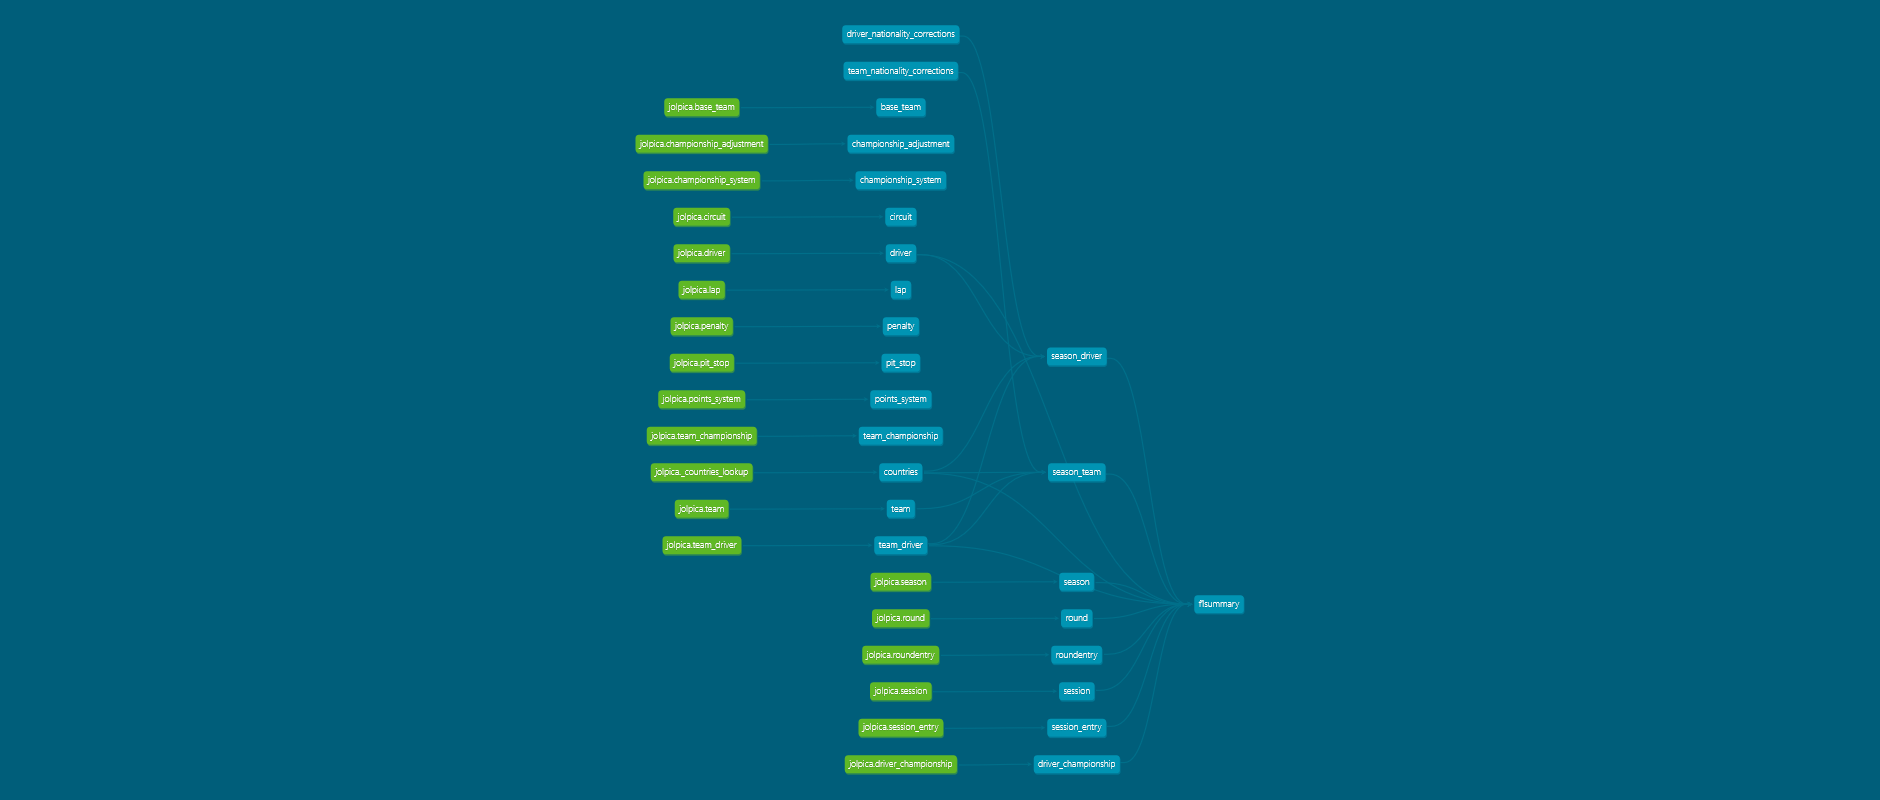
\includegraphics[width=1\linewidth]{../images/report/dbt-dag} 

}

\caption{Transformation lineage: Jolpica source tables (left) mapped through dbt to the analytical tables (right). This figure is a snapshot; the full, interactive and always up-to-date diagram is available in the project's online dbt documentation.}\label{fig:unnamed-chunk-57}
\end{figure}

Two observations about the shape of this graph summarise the philosophy
of Section 3.1. First, the large majority of source tables map
one-to-one to their analytical counterparts with no intermediate logic:
they are renamed, stripped of \texttt{api\_id}, and passed through.
Second, the deviations from this pattern are few and concentrated ---
the nationality corrections feed two dedicated tables, the external
fastest-lap source feeds the enriched results model, and a single
derived view exists at present. The transformation layer is
intentionally thin, and it is expected to grow slowly: as new analytical
views are added, the online documentation will diverge from the snapshot
reproduced here, which is precisely why the authoritative version is
published alongside the dbt-generated documentation rather than frozen
in this document.

\newpage

\subsection{\texorpdfstring{3.3 Removing the \texttt{api\_id}
Columns}{3.3 Removing the api\_id Columns}}\label{removing-the-api_id-columns}

As established in Section 2.4.2, every table of the export begins with
an \texttt{api\_id} column that identifies records within Jolpica's own
infrastructure but carries no analytical meaning. All such columns are
dropped during the staging step. The removal is purely structural --- it
affects no values, no joins and no row counts --- and is verified by the
row-count checks described in Section 2.2.

It should be stressed that this is a \textbf{deferral, not a rejection},
of the underlying information. Should a need ever arise to trace
analytical records back to Jolpica's API endpoints --- for example, for
debugging the extraction process or reconciling against future revisions
of the dump --- the original identifiers can be recovered from the raw
SQLite snapshot, which is itself version-controlled and distributed with
the pipeline. Introducing dedicated application-level lookup tables now
would add joins and maintenance surface for a use case that does not
currently exist; the decision is therefore recorded here and revisited
only if that use case materialises.

\newpage

\subsection{3.4 Season-Scoped
Nationalities}\label{season-scoped-nationalities}

Section 2.4.10 documented the central limitation of the raw schema
regarding nationality: a single, current-day value is retrojected onto
the entire history of each driver and team, so that the 1950 Alfa Romeo
works outfit --- unambiguously Italian at the time --- is recorded as
Swiss, and drivers who competed under more than one nationality, such as
Bertrand Gachot, can exhibit only one of them.

Fixing this properly would mean recording the nationality of every
entity in every season. For roughly 800 drivers and several hundred
constructor entities spanning three quarters of a century, such a
complete mapping cannot be reliably constructed from public records, and
fabricating coverage would violate the principle of Section 3.1. The
transformation therefore takes a narrower and more honest form:

\begin{itemize}
\tightlist
\item
  the original \texttt{country\_code} attributes on \texttt{driver} and
  \texttt{team} are retained unchanged and continue to serve as the
  \textbf{default} nationality;
\item
  two dedicated correction tables,
  \texttt{driver\_nationality\_corrections} and
  \texttt{team\_nationality\_corrections}, associate a country with an
  entity \textbf{over an explicit season interval}
  (\texttt{season\_id\_start} to \texttt{season\_id\_end}), overlaying
  the default wherever a correction exists.
\end{itemize}

The resulting model restores temporal resolution exactly where it is
needed: a query about a driver's or team's nationality in a given season
resolves against the correction table first, and falls back to the
source value otherwise. Corrections are applied only to the cases
documented in Section 2.4.10 --- Alfa Romeo's Italian identity prior to
its post-war reorganisation, Renault's dual French/British identity, and
drivers with confirmed multi-nationality careers such as Gachot --- each
entry traceable to the historical evidence discussed in Chapter 2.

\begin{table}[!h]
\centering\begingroup\fontsize{8}{10}\selectfont

\resizebox{\ifdim\width>\linewidth\linewidth\else\width\fi}{!}{
\begin{tabular}[t]{rrrl}
\toprule
driver\_id & season\_id\_start & season\_id\_end & country\_code\\
\midrule
684 & 40 & 41 & FRA\\
\bottomrule
\end{tabular}}
\endgroup{}
\end{table}

\begin{table}[!h]
\centering\begingroup\fontsize{8}{10}\selectfont

\resizebox{\ifdim\width>\linewidth\linewidth\else\width\fi}{!}{
\begin{tabular}[t]{rrrll}
\toprule
team\_id & season\_id\_start & season\_id\_end & country\_code & name\\
\midrule
152 & 62 & 62 & GBR & Lotus Renault GP\\
1 & 1 & 2 & ITA & NA\\
1 & 30 & 36 & ITA & NA\\
\bottomrule
\end{tabular}}
\endgroup{}
\end{table}

The distinction from the raw schema is worth making explicit: where
Jolpica can only state what an entity's nationality \emph{is}, the
analytical schema can state what it \emph{was at the time of a given
season}. Temporal analyses of nationality built on \texttt{formula1.db}
now describe the 1950 Alfa Romeo entries as Italian, at the cost of a
single join and a documented, extendable correction mechanism.

\newpage

\subsection{3.5 Restoring Fastest-Lap Coverage,
1950--1957}\label{restoring-fastest-lap-coverage-19501957}

Section 2.4.7 located a precise coverage boundary in the source: the
\texttt{fastest\_lap\_rank} column is empty for every session before the
1958 season, because officially tracked fastest laps were not part of
the championship's recordkeeping before then. The irony highlighted
there --- that the seven drivers who jointly set the fastest lap at the
1954 British Grand Prix carry their 1/7-point award in \texttt{points}
but cannot be recognised by the dedicated column --- is preserved
verbatim by the pass-through philosophy of this chapter.

However, unlike the other quirks of Chapter 2, this gap is a genuine
\emph{absence} of data rather than a period-accurate encoding, and the
missing information is recoverable: an external dataset records the
fastest-lap achievers for the seasons 1950--1957. As part of the
imminent modifications to the pipeline, this external table will be
joined onto the results model, populating \texttt{fastest\_lap\_rank}
(and the related fastest-lap attributes) for the affected seasons. The
enrichment is applied exclusively where the source is empty, so the
original values from 1958 onwards remain untouched and traceable to
Jolpica; provenance of the enriched values is recorded separately, in
keeping with the audit practices of the pipeline.

For the shared-award cases of Section 2.4.6, the enrichment deliberately
records the joint achievement as it stands in the historical record
rather than electing a single fastest driver --- consistent with the
treatment of multi-winner races in Section 2.4.4.

With this change, fastest-lap coverage becomes complete across the
entire championship history, and the ``absent fastest lap'' ceases to be
a limitation of the analytical dataset --- while remaining faithfully
absent from the raw snapshot, which is never modified.

\newpage

\subsection{\texorpdfstring{3.6 A Convenience View:
\texttt{f1summary}}{3.6 A Convenience View: f1summary}}\label{a-convenience-view-f1summary}

The analytical schema is normalised: answering even a simple question
--- \emph{who finished where, in which car, scoring how many points?}
--- requires joining \texttt{session\_entry}, \texttt{round},
\texttt{season}, \texttt{circuit}, \texttt{driver}, \texttt{team} and
the nationality resolution logic of Section 3.4. Writing these joins
anew for every query or visualisation is error-prone and obscures the
analysis itself. To make day-to-day access to the dataset frictionless,
the transformation therefore includes \textbf{convenience views}: flat,
de-normalised tables that pre-resolve the most common joins and expose
the data ready for display.

The principal view is \texttt{f1summary}, one row per race result, whose
columns are listed below.

\begin{table}[!h]
\centering\begingroup\fontsize{9}{11}\selectfont

\begin{tabular}[t]{>{\raggedright\arraybackslash}p{4.5cm}>{\raggedright\arraybackslash}p{10cm}}
\toprule
Column & Description\\
\midrule
resultId & Unique identifier for each result\\
grid & The driver's starting grid position\\
positionOrder & The driver's finishing position in order\\
points & Points scored by the driver in the race\\
laps & Number of laps completed by the driver\\
rank & The rank of the driver's fastest lap\\
statusId & Foreign key to status.csv\\
year & The year of the race\\
round & The round number of the race in the season\\
circuit & The official name of the circuit\\
driverNationality & The driver's nationality\\
constructorName & The full name of the constructor\\
constructorNationality & The nationality of the constructor\\
status & A description of the finishing status\\
driverAge & The driver's age at the time of the race\\
driverName & The driver's full name\\
\bottomrule
\end{tabular}
\endgroup{}
\end{table}

An extract of the view illustrates the outcome: each row combines
result, context and human-readable attributes into a single,
display-ready record.

\begin{table}[!h]
\centering\begingroup\fontsize{9}{11}\selectfont

\resizebox{\ifdim\width>\linewidth\linewidth\else\width\fi}{!}{
\begin{tabular}[t]{rrrrllrl}
\toprule
resultId & positionOrder & points & year & circuit & driverName & driverAge & constructorName\\
\midrule
1 & 1 & 9 & 1950 & British Grand Prix & Nino Farina & 44 & Alfa Romeo\\
2 & 2 & 6 & 1950 & British Grand Prix & Luigi Fagioli & 52 & Alfa Romeo\\
3 & 3 & 4 & 1950 & British Grand Prix & Reg Parnell & 39 & Alfa Romeo\\
4 & 4 & 3 & 1950 & British Grand Prix & Yves Cabantous & 46 & Talbot-Lago\\
5 & 5 & 2 & 1950 & British Grand Prix & Louis Rosier & 45 & Talbot-Lago\\
6 & 6 & 0 & 1950 & British Grand Prix & Bob Gerard & 36 & ERA\\
\bottomrule
\end{tabular}}
\endgroup{}
\end{table}

Two details of the view deserve emphasis. First, the nationality columns
(\texttt{driverNationality}, \texttt{constructorNationality}) are
\textbf{not} a verbatim copy of the source attributes: they are resolved
through the season-scoped correction mechanism of Section 3.4, so the
1950 entries display Alfa Romeo as Italian rather than Swiss. This is
precisely the kind of logic that belongs inside a view rather than being
reimplemented (or forgotten) in every downstream query. Second, derived
attributes computed during transformation --- \texttt{driverAge} among
them --- appear alongside the raw passthrough columns, giving the view
everything needed for descriptive analysis without touching the
normalised tables.

The view is intentionally materialised as a thin projection over the
analytical tables rather than a replacement for them: any measure beyond
its fixed column set (per-lap timings, pit stops, championship
trajectories) still queries the underlying schema directly. As the
transformation layer grows, additional views following the same pattern
will be added; the online dbt documentation referenced in Section 3.2
remains the authoritative record of what currently exists.

\newpage

\subsection{3.7 The Resulting Schema}\label{the-resulting-schema}

The outcome of the transformation is the analytical database
\texttt{formula1.db}, whose structure is shown below. The raw tables
appear in the schema largely unchanged, grouped by domain; the additions
of Section 3.4 are visible as the two
\texttt{*\_nationality\_corrections} tables together with the
\texttt{countries} lookup, and the season-scoped \texttt{season\_driver}
and \texttt{season\_team} associations.

\begin{figure}

{\centering 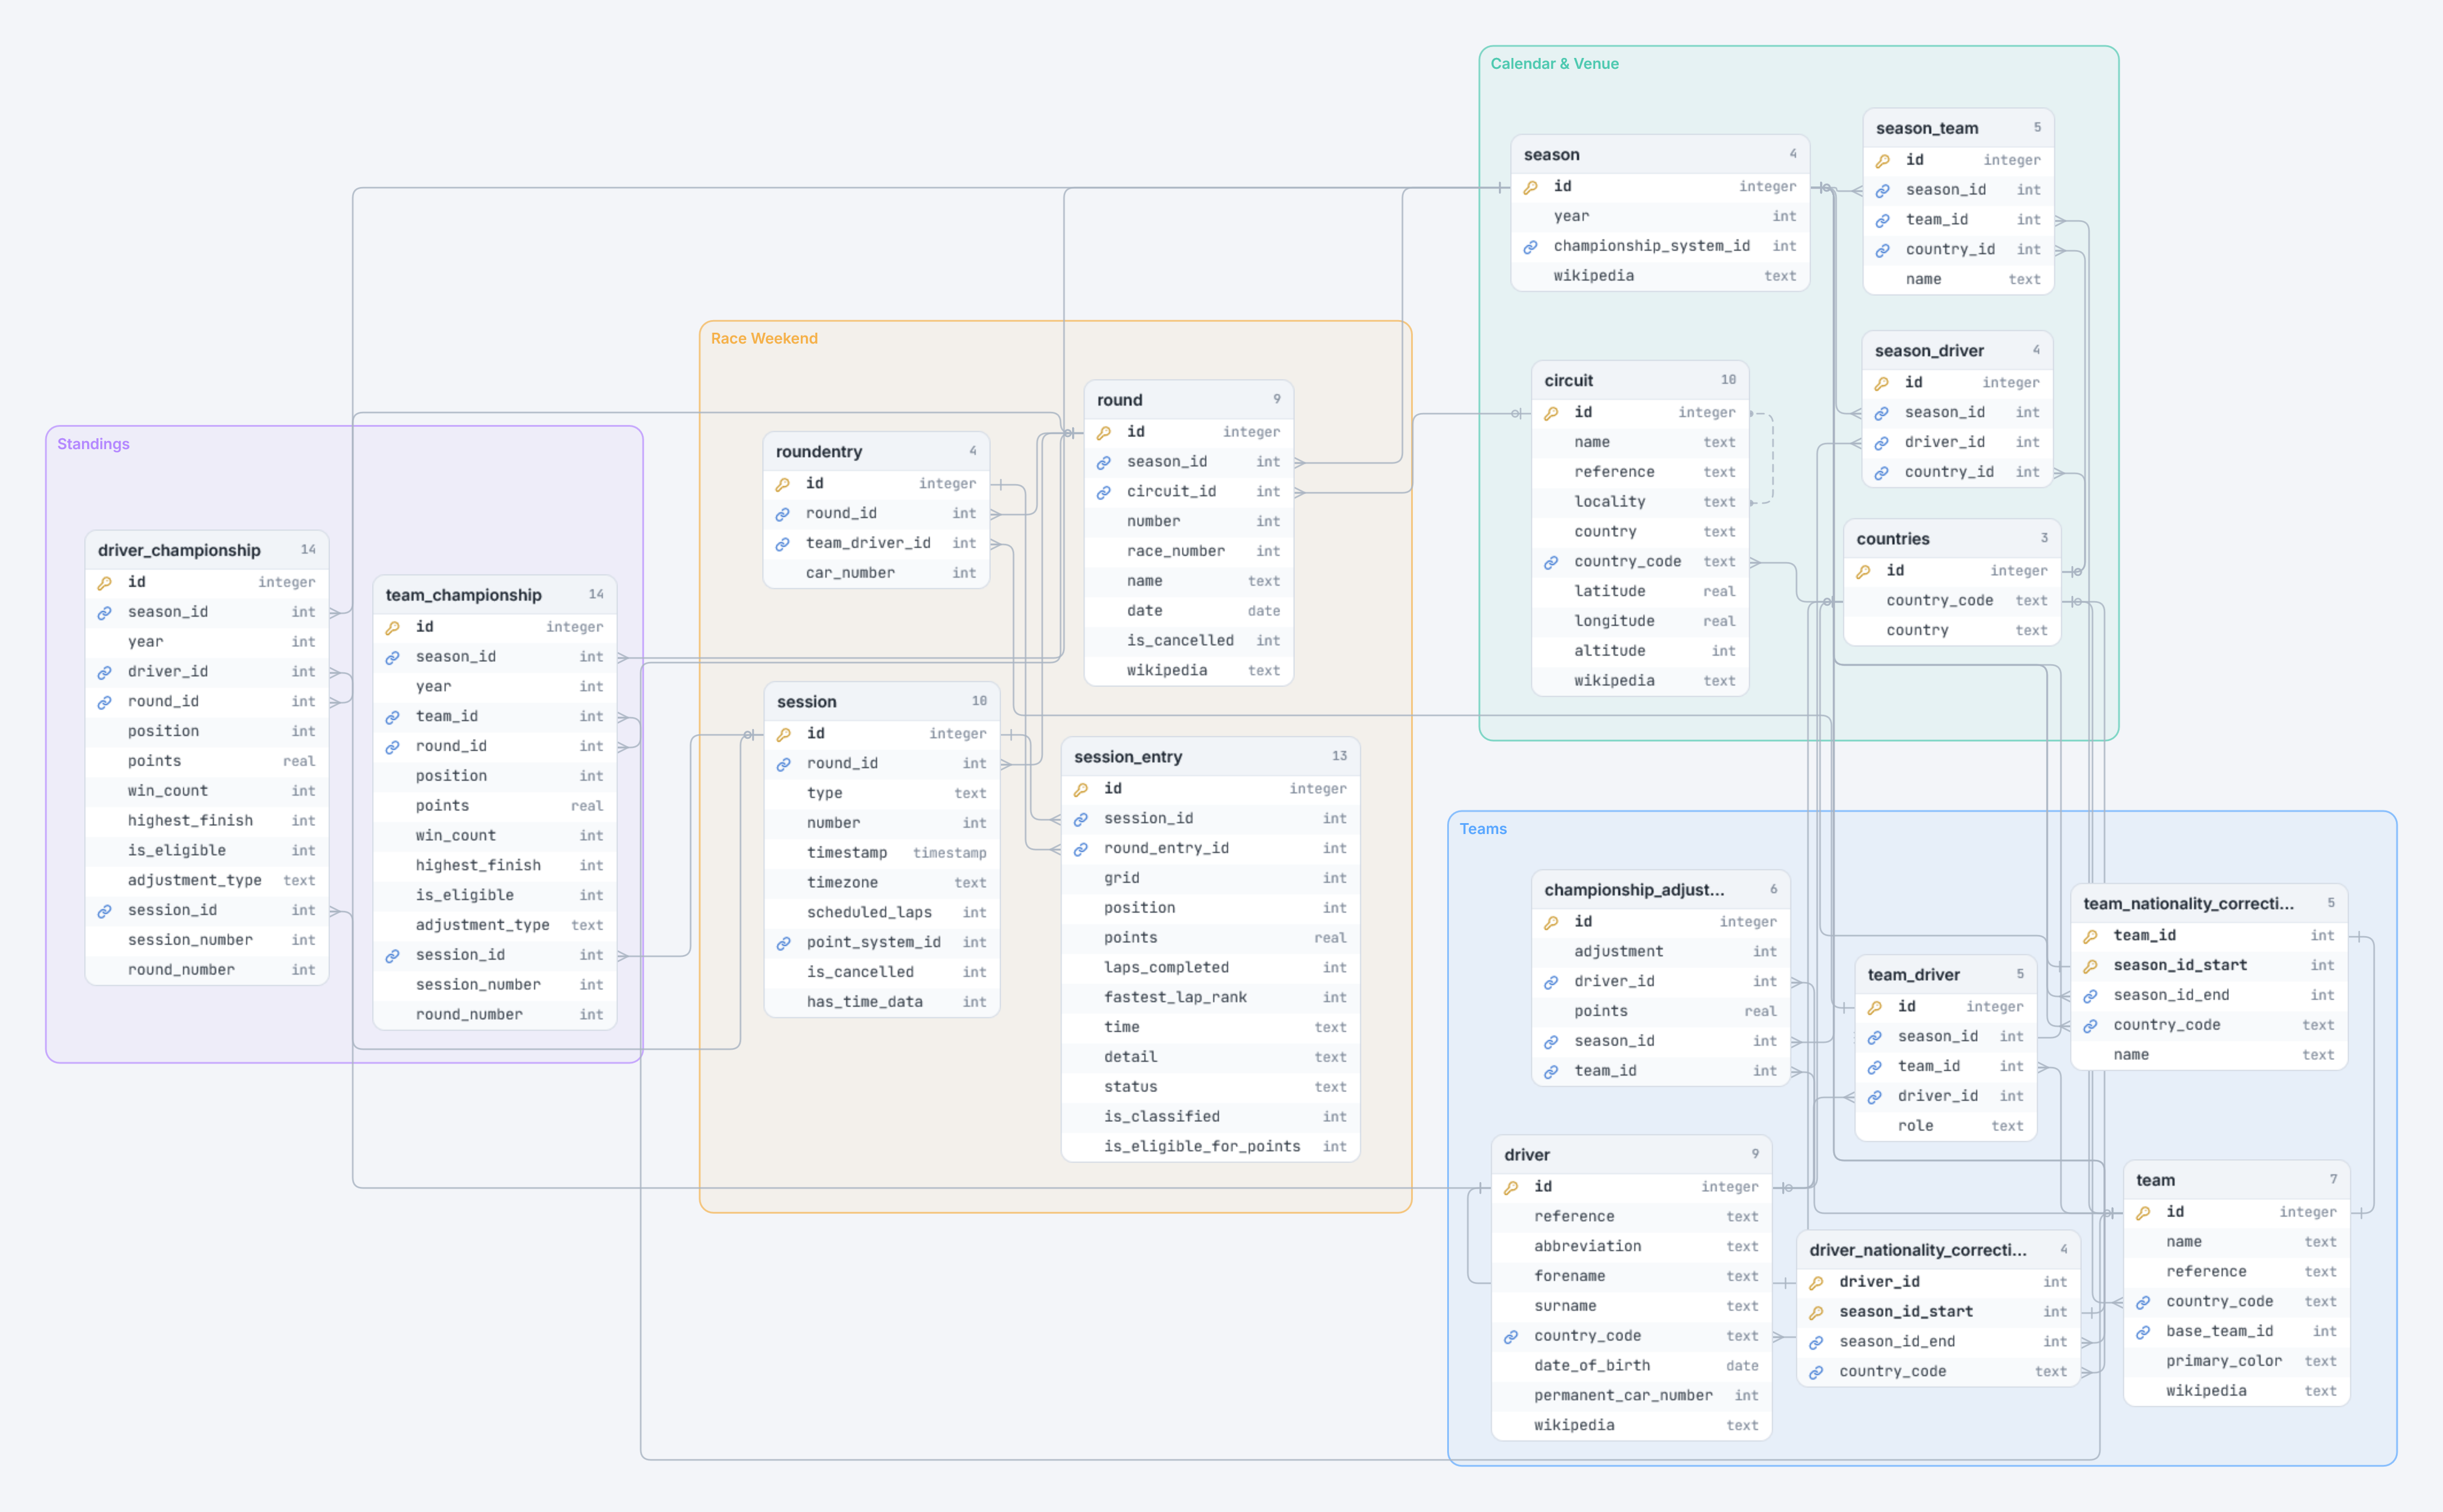
\includegraphics[width=1\linewidth]{../images/report/formula1_erd} 

}

\caption{Entity-relationship diagram of the analytical database `formula1.db` after transformation.}\label{fig:unnamed-chunk-62}
\end{figure}

\newpage

\subsection{3.8 What Is Deliberately Not
Changed}\label{what-is-deliberately-not-changed}

Completeness requires stating the inverse of the preceding sections: the
anomalies of Chapter 2 that survive the transformation \textbf{on
purpose}.

The multiple-winner races arising from shared drives (Section 2.4.3) and
the fractional points they produce (Section 2.4.6) are preserved as-is;
any ``deduplication'' would erase the only record that several drivers
jointly achieved a result. The driver whose eligibility flag contradicts
a positive point total (Section 2.4.8) is likewise preserved --- the
combination of \texttt{is\_eligible\_for\_points} and the notional point
share encodes a genuine period regulation, and separating the two
columns would lose it. Unclassified drivers carrying a fastest-lap point
(Section 2.4.9) are retained, including the singular case of Stirling
Moss at the 1959 French Grand Prix. Finally, the legacy
\texttt{roundentry} linkage and the empty staging tables
(\texttt{base\_team}, \texttt{penalty}) are carried through unchanged:
they cost nothing, document the source's own evolution, and removing
them would couple the analytical schema to assumptions about Jolpica's
future development.

Further integrity inconsistencies identified in Chapter 2 that do not
admit a verified correction at present are explicitly deferred: as with
the application-level identifier lookup tables of Section 3.3, the
guiding rule is that a documented limitation is preferable to a silent
or speculative ``fix''. The corrections mechanism of Section 3.4 and the
enrichment of Section 3.5 establish the pattern by which such fixes will
be introduced as evidence becomes available --- narrowly scoped,
individually documented, and never at the expense of the raw snapshot.

\newpage

\section{4. Exploratory Data Analysis}\label{exploratory-data-analysis}

This chapter explores the dataset along three levels, each one stepping
back from the raw record book. We first examine the drivers and the
achievements they accumulated --- titles, wins, careers. We then turn to
the constructors, whose cars set the ceiling under which those
achievements were earned. Finally, we examine the championship framework
itself --- the calendar and the scoring rules --- and show that any
comparison of drivers across eras must first neutralize how much the
framework has changed.

\subsection{4.1 Drivers}\label{drivers}

\subsubsection{4.1.1 Grand Prix}\label{grand-prix}

The formula 1 world championship started in 1950, and has been held
since then with no interruption. As of 2026, 76 seasons has been held,
with 1,149 races where 817 drivers were involved. Only 115 won a race,
and 35 won the world champion title :

\begin{table}[!h]
\centering\begingroup\fontsize{9}{11}\selectfont

\begin{tabular}[t]{>{\raggedleft\arraybackslash}p{2cm}>{\raggedleft\arraybackslash}p{2cm}>{\raggedleft\arraybackslash}p{2cm}>{\raggedleft\arraybackslash}p{2cm}>{\raggedleft\arraybackslash}p{2cm}}
\toprule
Number of Seasons & Number of Races & Number of Drivers & Number of Winners & Number of Champions\\
\midrule
76 & 1,149 & 817 & 115 & 35\\
\bottomrule
\end{tabular}
\endgroup{}
\end{table}

Out of the 35 world champions, 17 of them won the title several times.
The plots below show the number of drivers per title or win category :

\begin{figure}

{\centering 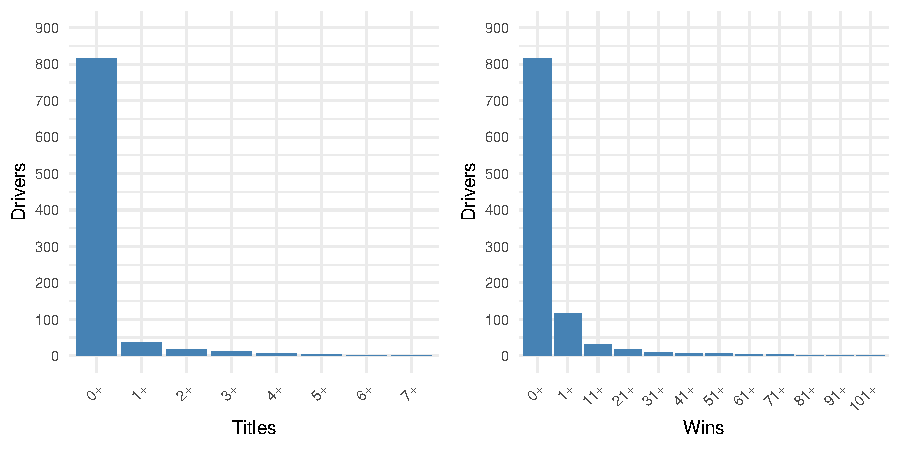
\includegraphics{Formula1_files/figure-latex/unnamed-chunk-74-1} 

}

\caption{Number of Titles or Wins per Driver}\label{fig:unnamed-chunk-74}
\end{figure}

\newpage

If we remove the drivers who didn't win any title or Grand Prix, we can
see the distinction in the plots below :

\begin{figure}

{\centering 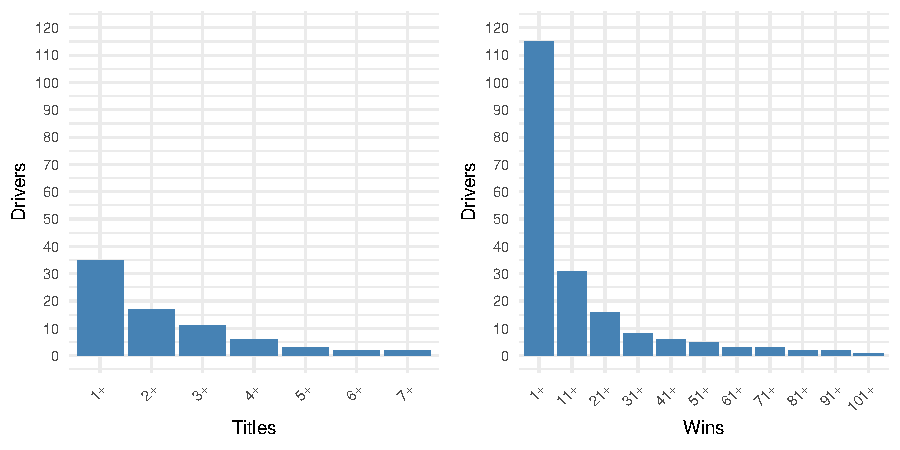
\includegraphics{Formula1_files/figure-latex/unnamed-chunk-75-1} 

}

\caption{Number of Titles or Wins per Driver (who won at least one race or title)}\label{fig:unnamed-chunk-75}
\end{figure}

The plots above show that most drivers didn't win any title. For those
who won at least one, half won only one title while the other won 2 or
more titles.

Very few drivers were able to become world champion while winning less
than 11 Grand prix in their whole career, and with no surprise they were
all competing in the early years, the most recent title being won by
Keke Rosberg in 1982, Rosberg who won 5 Grand Prix in his whole career :

\begin{table}[!h]
\centering\begingroup\fontsize{9}{11}\selectfont

\begin{tabular}{lrrl}
\toprule
driverName & titles & wins & year\\
\midrule
\includegraphics[width=0.25cm]{/home/runner/work/Formula-1/Formula-1/images/flags/icons8-italy-50.png} Nino Farina & 1 & 5 & 1950\\
\includegraphics[width=0.25cm]{/home/runner/work/Formula-1/Formula-1/images/flags/icons8-great-britain-50.png} Mike Hawthorn & 1 & 3 & 1958\\
\includegraphics[width=0.25cm]{/home/runner/work/Formula-1/Formula-1/images/flags/icons8-usa-50.png} Phil Hill & 1 & 3 & 1961\\
\includegraphics[width=0.25cm]{/home/runner/work/Formula-1/Formula-1/images/flags/icons8-great-britain-50.png} John Surtees & 1 & 6 & 1964\\
\includegraphics[width=0.25cm]{/home/runner/work/Formula-1/Formula-1/images/flags/icons8-new-zealand-50.png} Denny Hulme & 1 & 8 & 1967\\
\includegraphics[width=0.25cm]{/home/runner/work/Formula-1/Formula-1/images/flags/icons8-austria-50.png} Jochen Rindt & 1 & 6 & 1970\\
\includegraphics[width=0.25cm]{/home/runner/work/Formula-1/Formula-1/images/flags/icons8-great-britain-50.png} James Hunt & 1 & 10 & 1976\\
\includegraphics[width=0.25cm]{/home/runner/work/Formula-1/Formula-1/images/flags/icons8-south-africa-50.png} Jody Scheckter & 1 & 10 & 1979\\
\includegraphics[width=0.25cm]{/home/runner/work/Formula-1/Formula-1/images/flags/icons8-finland-50.png} Keke Rosberg & 1 & 5 & 1982\\
\bottomrule
\end{tabular}
\endgroup{}
\end{table}

On the other side, we also have drivers who, while winning many races
(more than 10), didn't win any title. The list below shows that, unlike
for the low-wins world champions, some of them were competing in the
early years of the F1. Notably, Carlos Reutemann and above all, Stirling
Moss won 16 Grand Prix over a career of 11 years starting in 1951 and
ending in 1961. As a comparison the champion Fangio won 24 races and 5
titles at the same period (1950-1958) :

\begin{table}[!h]
\centering\begingroup\fontsize{9}{11}\selectfont

\begin{tabular}{lrllr}
\toprule
driverName & wins & careerstart & careerend & careerlength\\
\midrule
\includegraphics[width=0.25cm]{/home/runner/work/Formula-1/Formula-1/images/flags/icons8-great-britain-50.png} Stirling Moss & 16 & 1951 & 1961 & 11\\
\includegraphics[width=0.25cm]{/home/runner/work/Formula-1/Formula-1/images/flags/icons8-argentina-50.png} Carlos Reutemann & 12 & 1972 & 1982 & 11\\
\includegraphics[width=0.25cm]{/home/runner/work/Formula-1/Formula-1/images/flags/icons8-brazil-50.png} Rubens Barrichello & 11 & 1993 & 2011 & 19\\
\includegraphics[width=0.25cm]{/home/runner/work/Formula-1/Formula-1/images/flags/icons8-great-britain-50.png} David Coulthard & 13 & 1994 & 2008 & 15\\
\includegraphics[width=0.25cm]{/home/runner/work/Formula-1/Formula-1/images/flags/icons8-brazil-50.png} Felipe Massa & 11 & 2002 & 2017 & 15\\
\bottomrule
\end{tabular}
\endgroup{}
\end{table}

\subsection{4.1.2 Winning Probability}\label{winning-probability}

\begin{figure}

{\centering 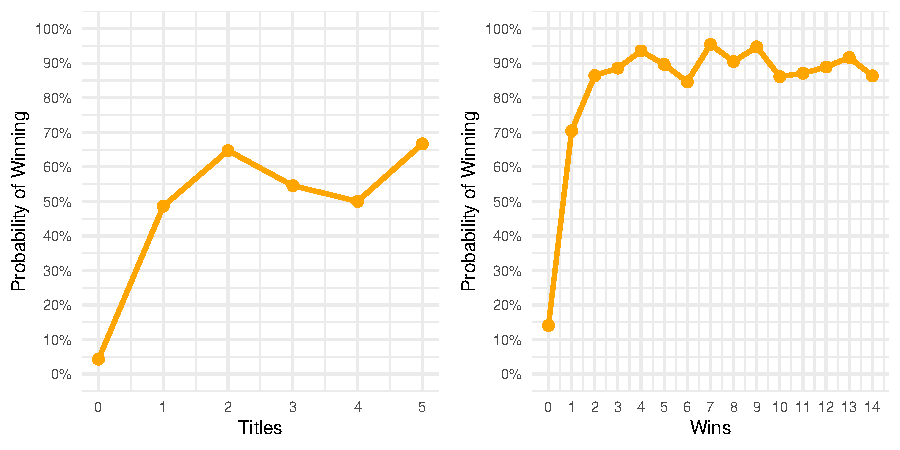
\includegraphics{Formula1_files/figure-latex/unnamed-chunk-78-1} 

}

\caption{Probability of Winning}\label{fig:unnamed-chunk-78}
\end{figure}

The ploys above show that the probability of winning is very low for
drivers who didn't win a title, and stays about 50\% for the other ones.
So each time a driver wins a title, he has 50\% of chances to win
another one. The 100\% probability at 6 titles is not very accurate
given the low number of drivers who won more than 5 titles (only 3
including Fangio).

\subsubsection{4.1.3 Top Drivers}\label{top-drivers}

If we define the leading drivers as those with the highest number of
titles, and among those who are world champions with an equal number of
titles, we can use the number of wins to differentiate them. This
results in the following table displaying the 17 drivers who won at
least 2 titles (as of 2025) :

\begin{table}[!h]
\centering\begingroup\fontsize{9}{11}\selectfont

\begin{tabular}{lrrrrrrr}
\toprule
driverName & titles & wins & races & seasons & points & titlespc & winspc\\
\midrule
\includegraphics[width=0.25cm]{/home/runner/work/Formula-1/Formula-1/images/flags/icons8-great-britain-50.png} Lewis Hamilton & 7 & 105 & 380 & 19 & 4,955.50 & 0.368 & 0.276\\
\includegraphics[width=0.25cm]{/home/runner/work/Formula-1/Formula-1/images/flags/icons8-germany-50.png} Michael Schumacher & 7 & 91 & 308 & 19 & 1,566.00 & 0.368 & 0.295\\
\includegraphics[width=0.25cm]{/home/runner/work/Formula-1/Formula-1/images/flags/icons8-argentina-50.png} Juan Fangio & 5 & 24 & 58 & 8 & 279.14 & 0.625 & 0.414\\
\includegraphics[width=0.25cm]{/home/runner/work/Formula-1/Formula-1/images/flags/icons8-netherlands-50.png} Max Verstappen & 4 & 71 & 233 & 11 & 3,301.50 & 0.364 & 0.305\\
\includegraphics[width=0.25cm]{/home/runner/work/Formula-1/Formula-1/images/flags/icons8-germany-50.png} Sebastian Vettel & 4 & 53 & 300 & 16 & 3,098.00 & 0.250 & 0.177\\
\includegraphics[width=0.25cm]{/home/runner/work/Formula-1/Formula-1/images/flags/icons8-france-50.png} Alain Prost & 4 & 51 & 202 & 13 & 798.50 & 0.308 & 0.252\\
\includegraphics[width=0.25cm]{/home/runner/work/Formula-1/Formula-1/images/flags/icons8-brazil-50.png} Ayrton Senna & 3 & 41 & 161 & 11 & 614.00 & 0.273 & 0.255\\
\includegraphics[width=0.25cm]{/home/runner/work/Formula-1/Formula-1/images/flags/icons8-great-britain-50.png} Jackie Stewart & 3 & 27 & 100 & 9 & 360.00 & 0.333 & 0.270\\
\includegraphics[width=0.25cm]{/home/runner/work/Formula-1/Formula-1/images/flags/icons8-austria-50.png} Niki Lauda & 3 & 25 & 173 & 13 & 420.50 & 0.231 & 0.145\\
\includegraphics[width=0.25cm]{/home/runner/work/Formula-1/Formula-1/images/flags/icons8-brazil-50.png} Nelson Piquet & 3 & 23 & 205 & 14 & 485.50 & 0.214 & 0.112\\
\includegraphics[width=0.25cm]{/home/runner/work/Formula-1/Formula-1/images/flags/icons8-australia-50.png} Jack Brabham & 3 & 14 & 129 & 16 & 261.00 & 0.188 & 0.109\\
\includegraphics[width=0.25cm]{/home/runner/work/Formula-1/Formula-1/images/flags/icons8-spain-50.png} Fernando Alonso & 2 & 32 & 428 & 22 & 2,380.00 & 0.091 & 0.075\\
\includegraphics[width=0.25cm]{/home/runner/work/Formula-1/Formula-1/images/flags/icons8-great-britain-50.png} Jim Clark & 2 & 25 & 73 & 9 & 274.00 & 0.222 & 0.342\\
\includegraphics[width=0.25cm]{/home/runner/work/Formula-1/Formula-1/images/flags/icons8-finland-50.png} Mika Häkkinen & 2 & 20 & 163 & 11 & 420.00 & 0.182 & 0.123\\
\includegraphics[width=0.25cm]{/home/runner/work/Formula-1/Formula-1/images/flags/icons8-brazil-50.png} Emerson Fittipaldi & 2 & 14 & 146 & 11 & 281.00 & 0.182 & 0.096\\
\includegraphics[width=0.25cm]{/home/runner/work/Formula-1/Formula-1/images/flags/icons8-great-britain-50.png} Graham Hill & 2 & 14 & 177 & 18 & 289.00 & 0.111 & 0.079\\
\includegraphics[width=0.25cm]{/home/runner/work/Formula-1/Formula-1/images/flags/icons8-italy-50.png} Alberto Ascari & 2 & 13 & 36 & 6 & 140.14 & 0.333 & 0.361\\
\bottomrule
\end{tabular}
\endgroup{}
\end{table}

For each driver, we observe the number of titles, total races won, total
races competed, the number of seasons or years they participated, the
total points earned (only those that count toward the championship), the
ratio of titles to seasons, and the ratio of wins to races.

Although the number of titles and races won clearly shows that Michael
Schumacher and Lewis Hamilton outshine other drivers, the same is not
necessarily the case for points. When we rank drivers by points, both
Verstappen and Vettel surpass Schumacher. Even Alonso who won 2 titles,
compared with the 7 by Schumacher, has more points than the latter.

To add another layer of complexity, if we look at the ratio of titles to
seasons or the ratio of wins to races, Juan Manuel Fangio emerges as the
top performer. Even Ascari, who appears at the bottom of the list, has
the second best ratio win to races.

Now if we look at the first 9 pilots, only 2 of them (Fangio and
Stewart) were racing at the earliest days of Formula 1. On the opposite,
if we look at the last 8 drivers, 4 of them were driving at the earliest
days : Brabham, Clark, Hill and Ascari. We can also notice that most of
these early drivers had a career under 10 years, when modern days
drivers have a career that last more than 10 years if not 20. Only
notable exception is Graham Hill who had a long career of 18 years from
1958 to 1975.

We will now see the careers and titles of these 17 drivers across the
years.

\newpage

\subsubsection{4.1.4 Timeline}\label{timeline}

The plot below illustrates the duration and timeline of careers without
indicating any breaks; for instance, Alain Prost did not compete in
1992, and Schumacher was absent from the tracks from 2007 to 2009.

\begin{figure}

{\centering 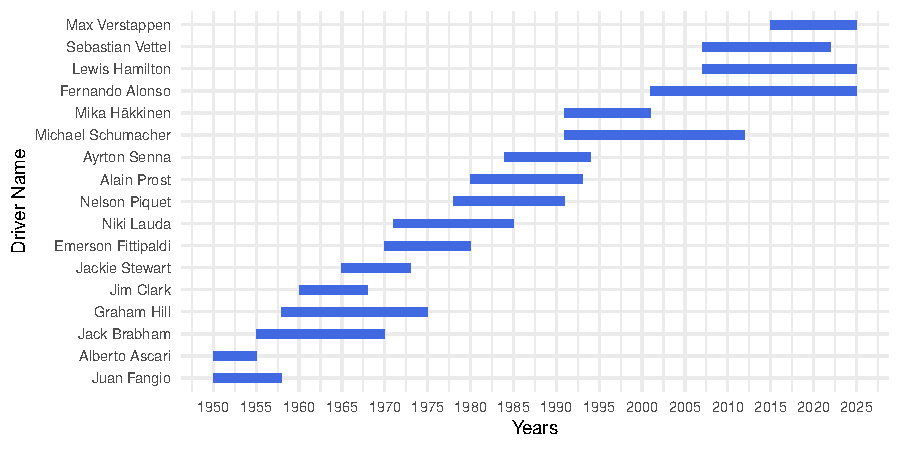
\includegraphics{Formula1_files/figure-latex/unnamed-chunk-80-1} 

}

\caption{Careers}\label{fig:unnamed-chunk-80}
\end{figure}

Some drivers enjoyed longer careers than others. For instance, Alonso,
Schumacher, and Hamilton had the longest career spans, while Ascari,
Clark, and Stewart had the shortest. The problem with this graph is that
it does not effectively depict the dominance of any particular driver.
For instance, Alonso secured his two titles in 2005 and 2006, and has
continued racing since without winning any additional titles.

Now, if we replace the career duration with titles, where each segment
represents the years between a driver's first and last title, we obtain
the following graph :

\begin{figure}

{\centering 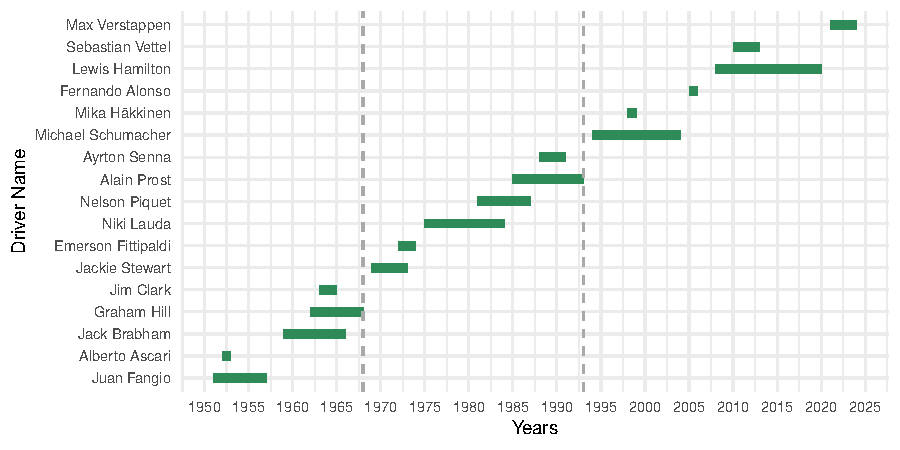
\includegraphics{Formula1_files/figure-latex/unnamed-chunk-81-1} 

}

\caption{Titles}\label{fig:unnamed-chunk-81}
\end{figure}

We divided this timeline into three phases: the first phase, the early
stage, extends from the beginning until the late 1960s. The second phase
begins with Jackie Stewart's first title in 1969 and continues until
Michael Schumacher's first title in 1994. The final phase, or modern
era, starts in 1994 and continues to the present.

In the plot above, each phase is marked with a vertical dashed grey
line.

Now, when we display the career lengths based on the year of the first
title, we can observe a gradual increase over the years :

\begin{figure}

{\centering 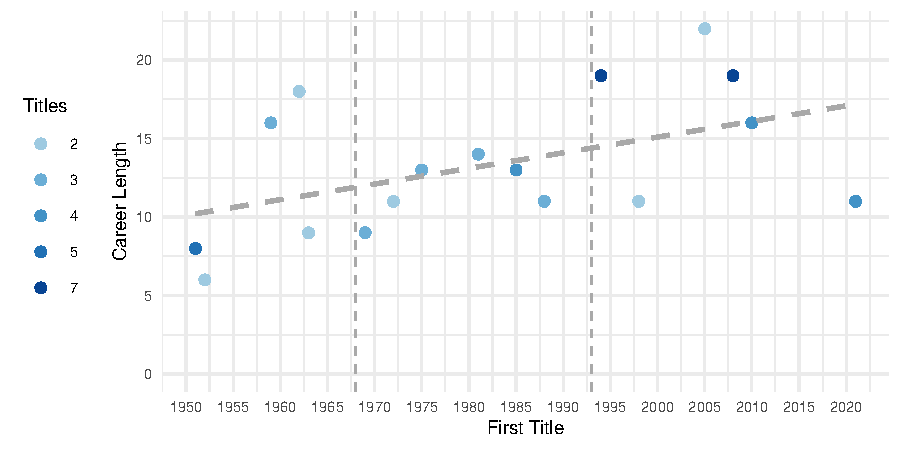
\includegraphics{Formula1_files/figure-latex/unnamed-chunk-82-1} 

}

\caption{Career Start vs Career Length}\label{fig:unnamed-chunk-82}
\end{figure}

A clear upward trend emerges, suggesting that drivers who started their
careers in more recent decades tend to have longer careers. This may be
attributed to various factors, including advancements in safety,
improvements in car technology, and changes in race formats that allow
for prolonged competition. Notable drivers in the modern era, such as
Hamilton, benefit from these advancements, resulting in extended careers
compared to drivers from earlier periods.

We can notice that while Juan Manuel Fangio was able to secure 5 titles
within 8 years in the 1950s, Michael Schumacher and Lewis Hamilton
achieved their 7 titles in 19 and 20 years respectively, with Hamilton
still actively competing. This illustrates how the demands and dynamics
of racing have shifted over time. The differentiation of data points by
title count adds another layer of insight. Drivers with more titles,
represented by larger and darker-colored points, typically have career
lengths that align with the observed trend. The correlation suggests
that those who excel and secure multiple championships also tend to
enjoy longer careers, potentially due to their consistent performance,
adaptability, and resilience in the competitive environment.

Conversely, while some historical drivers achieved significant success
in fewer years, many of them faced different challenges, such as fewer
races per season and a more hazardous racing environment. This context
helps explain why earlier drivers, despite their talent, often have
shorter career lengths represented in the plot.

The dashed line in the graph indicates the overall trend, reinforcing
the notion that career length has increased over time for Formula 1
drivers. This trend not only reflects the effects of improved safety and
technology but may also point to changes in how drivers manage their
careers, including fitness and approach to racing.

\newpage

\subsubsection{4.1.5 Comparison}\label{comparison}

Now, let's compare the top drivers based on their wins and the number of
races they have participated in :

\begin{figure}

{\centering 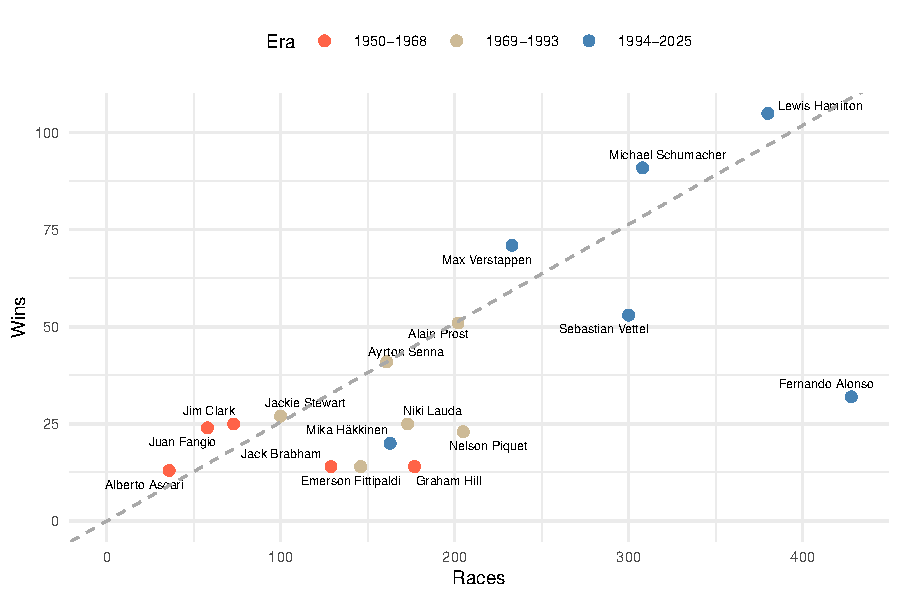
\includegraphics{Formula1_files/figure-latex/unnamed-chunk-83-1} 

}

\caption{Wins vs Races}\label{fig:unnamed-chunk-83}
\end{figure}

There is a noticeable upward trend in the plot, suggesting that drivers
who participate in more races tend to achieve a higher number of wins.
This correlation implies that experience and track time significantly
contribute to success in the sport. Drivers from the 1994 to 2023 era,
such as Hamilton and Vettel, are positioned in the top right quadrant,
indicating both a high number of races and wins. The representation of
this era in a distinct color underscores the advantages of modern
technology and greater competitiveness, reflecting a notable shift in
performance standards.

The varying colors used to group drivers by era emphasize the
differences in victory rates and opportunities for success across time.
Historical drivers may have achieved fewer wins but did so in a context
with fewer races and different competitive landscapes. For instance,
earlier eras, represented in warmer colors, often had fewer wins despite
high title counts, pointing to the unique challenges faced by those
drivers. Additionally, Fernando Alonso stands out for having a
considerable number of races with only two titles, highlighting that a
lengthy career does not guarantee championship success. This suggests
that various external factors, such as team dynamics and competitive
context, play significant roles in determining outcomes.

Overall, the plot illustrates that while participation in a greater
number of races can lead to more wins, it does not exclusively dictate a
driver's success. Factors like team performance, car technology, and the
competitiveness of each era are crucial. The shifts in driver success
across different decades indicate an evolution in Formula 1, influenced
by changes in race formats and team strategies, as well as an expanding
global audience. The color-coded groupings serve to highlight how
drivers' experiences and achievements are shaped by the specific
challenges and opportunities of their respective eras. This analysis
provides a thorough understanding of the factors influencing driver
success in Formula 1, as visualized through the plot, while also
acknowledging the historical context that contributes to these
differences.

\newpage

And now the number of titles and seasons per driver :

\begin{figure}

{\centering 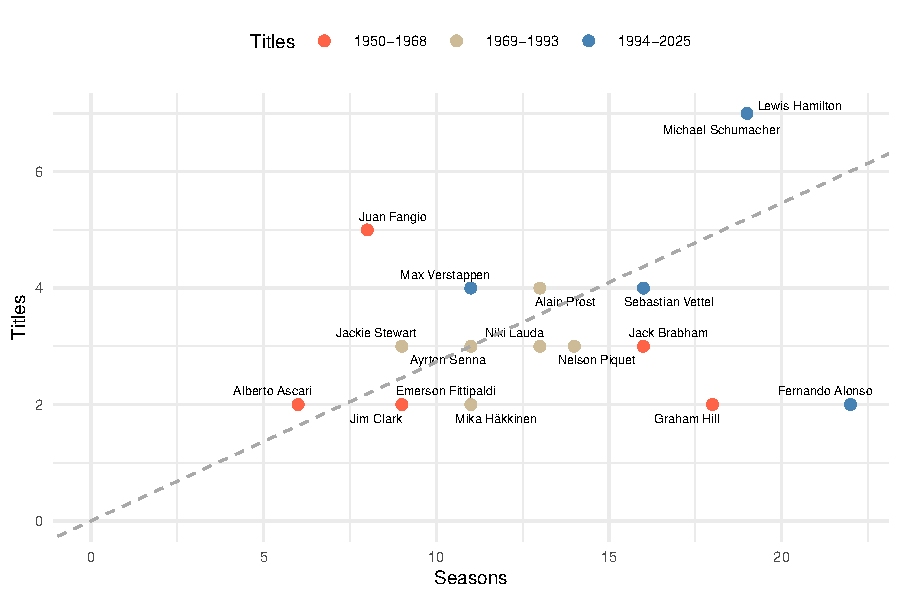
\includegraphics{Formula1_files/figure-latex/unnamed-chunk-84-1} 

}

\caption{Titles vs Seasons}\label{fig:unnamed-chunk-84}
\end{figure}

While the plot displays a trend where drivers with more seasons tend to
win multiple titles, this is true for those who have achieved two or
more titles. Notably, modern drivers such as Hamilton and Vettel,
positioned in the top right quadrant, exemplify this trend, showcasing
the advantage of extended careers combined with high performance. Their
achievements in more recent years highlight the advancements in
technology and team strategies that have influenced competitive
outcomes.

The color coding of the data points emphasizes differences in
performance across historical eras. For instance, drivers from the 1950
to 1988 timeframe, such as Fangio and Clark, achieved multiple titles
within fewer seasons, reflecting the unique challenges of their
competitive environments, which often had fewer races and different
dynamics compared to today. This juxtaposition illustrates how the
number of titles can vary significantly based on the era in which the
drivers competed.

Additionally, the representation of drivers like Alonso showcases the
relationship between seasons and titles, as he has spent a considerable
number of seasons in the sport but has only two titles. This highlights
that having a long career does not always correlate with championship
victories, suggesting the impact of factors like team performance,
adaptability, and the competitive landscape at any given time.

Overall, the plot underscores that while participation in more seasons
can lead to multiple titles, it does not guarantee success. Various
factors, including team dynamics, technological advancements, and the
competitive environment in different eras, play crucial roles in
determining a driver's achievements. The shifts in performance across
different decades indicate an evolution within Formula 1, influenced by
changing race formats and an increasingly global audience. This analysis
provides a comprehensive understanding of how the number of seasons
impacts title success while also recognizing the historical context that
shapes these outcomes.

\newpage

\subsubsection{4.1.6 Summary}\label{summary}

{[}We saw that recent drivers achieved better results with time, we also
saw that some drivers were able to achieve better or same results in a
shorter timeframe.

But this is not enough to determine if these drivers were really better
than others. Would Fangio have achieved 10 titles have he run 16
seasons? What about the variation of number of races, points and rules
over the seasons? And what about the car itself?{]}

We observed that recent drivers have generally achieved better results
over time, indicating a trend of improved performance in modern Formula
1. This improvement can be attributed to a variety of factors, including
advancements in technology, enhanced training practices, and improved
team dynamics. However, it is equally noteworthy that some drivers from
earlier eras managed to achieve comparable results within a
significantly shorter timeframe. This raises an important question
regarding the true measure of a driver's ability and whether career
longevity directly equates to skill or success on the race track.

To determine if these recent drivers are genuinely better than their
predecessors, we must consider multiple dimensions of comparison. For
instance, would Juan Manuel Fangio have achieved 10 titles if he had
raced for 16 seasons, similar to modern drivers? Fangio, who secured his
five titles in just eight years during the 1950s, faced vastly different
competitive landscapes and challenges than those in contemporary racing.
His remarkable success in such a brief period prompts an investigation
into context: how much of his success was due to his skill versus the
circumstances and limitations of his era?

Additionally, the evolution of the sport itself complicates these
comparisons. Over the years, Formula 1 has undergone significant changes
in terms of race formats, scoring systems, and regulations. The number
of races in a season has fluctuated, impacting a driver's opportunity to
accumulate wins and points. In some seasons, drivers competed in fewer
races, which naturally limits their chances for high totals, making it
essential to contextualize statistics within the framework of their
respective eras.

Points systems have also varied dramatically, altering how achievements
are measured. Modern scoring rewards consistency and resilience across
more races, which can skew comparisons against drivers from the past,
who may have excelled under a different set of rules. For instance,
Fangio's era awarded fewer points for victories, but achieving those
wins was often subject to harsher competition and racing conditions.

Moreover, the cars themselves represent a crucial aspect of this
discussion. The technology and engineering behind F1 cars have advanced
exponentially over the decades, with modern vehicles benefiting from
aerodynamics, data analysis, and materials that were not available in
the past. This raises another question: how much of a driver's success
is attributable to their talent and how much is due to the superior
performance of the car?

The answer, of course, is that no such verdict can be reached from raw
tallies alone. Would Juan Manuel Fangio have accumulated 10 titles had
he contested 16 seasons like a modern driver, instead of the 8 years
over which he collected his 5? The question sounds speculative, but its
premise is measurable: the number of races contested per season, the
points awarded for each result, and the number of seasons over which a
career could unfold all differ systematically between Fangio's era and
Hamilton's. A title count, a win count, or a points total is therefore
not a pure measure of ability --- it is a count of \emph{opportunities
converted}, and the number of opportunities on offer varied enormously
across the championship's history.

Before these quantities can be compared, one further confounder must be
acknowledged: none of the results catalogued above were achieved alone.
Every win and every title was earned in a car built by a constructor,
and the spread between the dominant machines and the rest has been wider
in some eras than in others. The next section therefore turns to the
constructors, whose fortunes bound those of the drivers they employ.

\newpage

\subsection{4.2 Constructors}\label{constructors}

The table below shows the number of constructors involved in the
championship over the years ;

\begin{table}[!h]
\centering\begingroup\fontsize{9}{11}\selectfont

\begin{tabular}[t]{>{\raggedleft\arraybackslash}p{2cm}>{\raggedleft\arraybackslash}p{2cm}>{\raggedleft\arraybackslash}p{2cm}>{\raggedleft\arraybackslash}p{2cm}}
\toprule
Number of Constructors & Points & Wins & Titles\\
\midrule
203 & 106 & 47 & 18\\
\bottomrule
\end{tabular}
\endgroup{}
\end{table}

As of 2025, 203 constructors participated in the world championships.
106 of them won at least one point, 47 won a race and 18 won a title.

And this is a list of the constructors who won the championship at least
once :

\begin{table}[!h]
\centering\begingroup\fontsize{9}{11}\selectfont

\begin{tabular}{lrrrllr}
\toprule
constructorName & titles & wins & points & start & end & seasons\\
\midrule
\includegraphics[width=0.25cm]{/home/runner/work/Formula-1/Formula-1/images/flags/icons8-italy-50.png} Ferrari & 22 & 249 & 11,451.27 & 1950 & 2025 & 76\\
\includegraphics[width=0.25cm]{/home/runner/work/Formula-1/Formula-1/images/flags/icons8-great-britain-50.png} McLaren & 11 & 199 & 7,797.50 & 1968 & 2025 & 56\\
\includegraphics[width=0.25cm]{/home/runner/work/Formula-1/Formula-1/images/flags/icons8-germany-50.png} Mercedes & 9 & 131 & 8,154.64 & 1954 & 2025 & 18\\
\includegraphics[width=0.25cm]{/home/runner/work/Formula-1/Formula-1/images/flags/icons8-great-britain-50.png} Williams & 9 & 114 & 3,765.00 & 1975 & 2025 & 50\\
\includegraphics[width=0.25cm]{/home/runner/work/Formula-1/Formula-1/images/flags/icons8-austria-50.png} Red Bull & 6 & 130 & 8,083.00 & 2005 & 2025 & 21\\
\includegraphics[width=0.25cm]{/home/runner/work/Formula-1/Formula-1/images/flags/icons8-great-britain-50.png} BRM & 3 & 17 & 537.50 & 1951 & 1977 & 23\\
\includegraphics[width=0.25cm]{/home/runner/work/Formula-1/Formula-1/images/flags/icons8-france-50.png} Renault & 2 & 35 & 1,777.00 & 1977 & 2020 & 24\\
\includegraphics[width=0.25cm]{/home/runner/work/Formula-1/Formula-1/images/flags/icons8-great-britain-50.png} Tyrrell & 2 & 23 & 711.00 & 1970 & 1998 & 29\\
\includegraphics[width=0.25cm]{/home/runner/work/Formula-1/Formula-1/images/flags/icons8-great-britain-50.png} Cooper-Climax & 2 & 12 & 336.50 & 1959 & 1968 & 9\\
\includegraphics[width=0.25cm]{/home/runner/work/Formula-1/Formula-1/images/flags/icons8-great-britain-50.png} Brabham-Repco & 2 & 8 & 175.00 & 1966 & 1969 & 4\\
\includegraphics[width=0.25cm]{/home/runner/work/Formula-1/Formula-1/images/flags/icons8-great-britain-50.png} Team Lotus & 1 & 45 & 995.00 & 1958 & 1994 & 29\\
\includegraphics[width=0.25cm]{/home/runner/work/Formula-1/Formula-1/images/flags/icons8-italy-50.png} Benetton & 1 & 27 & 861.50 & 1986 & 2001 & 16\\
\includegraphics[width=0.25cm]{/home/runner/work/Formula-1/Formula-1/images/flags/icons8-great-britain-50.png} Lotus-Climax & 1 & 22 & 281.00 & 1961 & 1967 & 7\\
\includegraphics[width=0.25cm]{/home/runner/work/Formula-1/Formula-1/images/flags/icons8-italy-50.png} Alfa Romeo & 1 & 11 & 361.00 & 1950 & 2023 & 16\\
\includegraphics[width=0.25cm]{/home/runner/work/Formula-1/Formula-1/images/flags/icons8-great-britain-50.png} Lotus-Ford & 1 & 11 & 209.00 & 1963 & 1971 & 5\\
\includegraphics[width=0.25cm]{/home/runner/work/Formula-1/Formula-1/images/flags/icons8-italy-50.png} Maserati & 1 & 9 & 313.42 & 1950 & 1960 & 11\\
\includegraphics[width=0.25cm]{/home/runner/work/Formula-1/Formula-1/images/flags/icons8-france-50.png} Matra-Ford & 1 & 9 & 130.00 & 1968 & 1969 & 2\\
\includegraphics[width=0.25cm]{/home/runner/work/Formula-1/Formula-1/images/flags/icons8-great-britain-50.png} Brawn & 1 & 8 & 172.00 & 2009 & 2009 & 1\\
\bottomrule
\end{tabular}
\endgroup{}
\end{table}

Ferrari stands out prominently with 22 titles and 249 wins, indicating a
dominant presence in the sport since 1950. McLaren and Mercedes follow,
with 11 and 9 titles respectively. Constructors like Williams and Red
Bull have also made significant contributions, evidenced by their
multiple wins and points. However, it's important to note that
constructors such as Mercedes and Alfa Romeo did not participate
consistently throughout the years. For instance, Mercedes withdrew from
racing after the 24h of Le Mans disaster in 1954 and returned to the
tracks only in 2010. Similarly, Alfa Romeo has had gaps in its
participation, despite its historical significance, which reflects the
varying levels of engagement among different teams over the decades.

\newpage

Now the constructors results over time. Comparison between constructors
who won most points from first to second :

\begin{figure}

{\centering 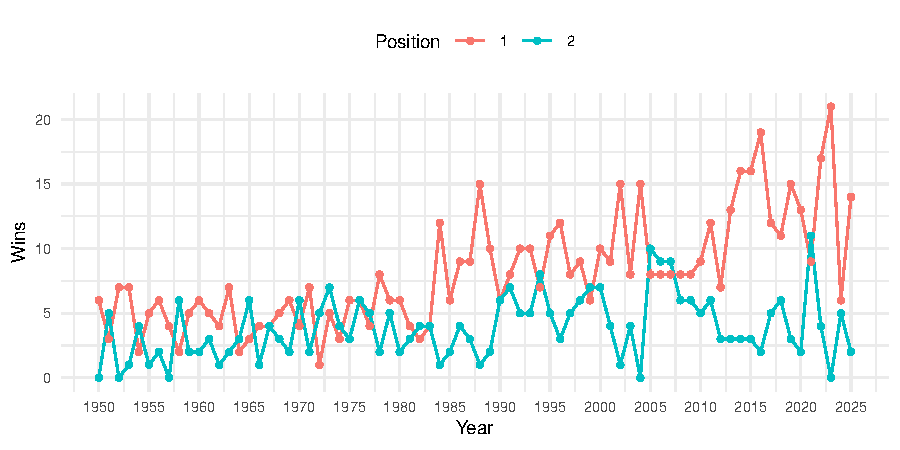
\includegraphics{Formula1_files/figure-latex/unnamed-chunk-87-1} 

}

\caption{Constructor Results}\label{fig:unnamed-chunk-87}
\end{figure}

And the driver results as a comparison :

\begin{figure}

{\centering 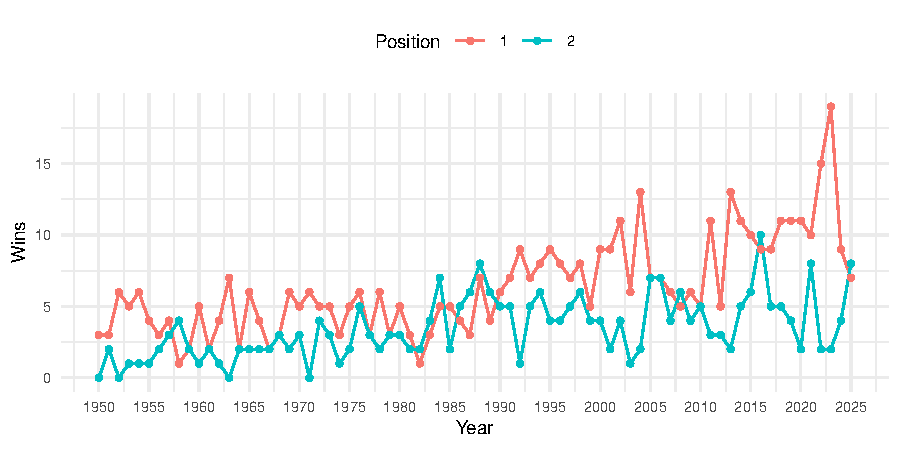
\includegraphics{Formula1_files/figure-latex/unnamed-chunk-88-1} 

}

\caption{Driver Results}\label{fig:unnamed-chunk-88}
\end{figure}

These trajectories make clear that a driver's record is partly a record
of the car beneath him. Fangio's 5 titles were won with four different
manufacturers --- a feat reflecting an era in which the field was
comparatively level --- while several modern champions collected titles
in long stretches of team dominance that no rival could match.
Participating in the right era of the right constructor can thus inflate
or deflate a driver's tally as surely as any change of rules. Yet even
controlling for the car does not level the playing field, because the
two frameworks in which every constructor and driver operated --- the
length of the calendar and the scoring system --- shifted repeatedly
across the decades. It is to these framework effects that the final
section of this chapter turns.

\newpage

\subsection{4.3 Championship Framework}\label{championship-framework}

\subsubsection{4.3.1 Races}\label{races}

The plot below illustrates the trend in the number of Formula 1 races
held each year from 1950 to 2023. The x-axis represents the year, while
the y-axis indicates the number of races. Each point reflects the actual
number of races for that specific year, depicted in gray, and the
variation among these points indicates fluctuations in race counts over
the years, reflecting changes in the racing calendar and external
factors affecting the sport.

\begin{figure}

{\centering 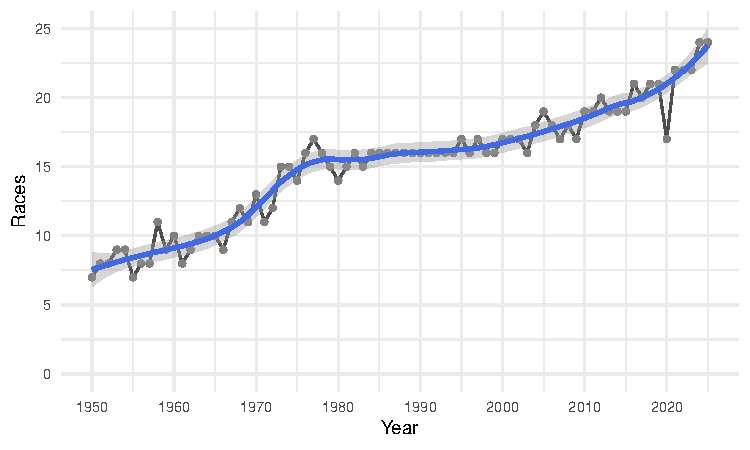
\includegraphics{Formula1_files/figure-latex/unnamed-chunk-89-1} 

}

\caption{Races per Year}\label{fig:unnamed-chunk-89}
\end{figure}

A clear upward trend is evident, starting from just 7 races in 1950 and
gradually increasing, with several plateaus extending into the late 20th
century. A more pronounced rise occurs in the 21st century, culminating
in approximately 23 races by 2023, suggesting the growing popularity and
expansion of Formula 1.

The loess smoothing curve, shown in royal blue, overlays the data points
to provide a clearer representation of the overall trend in race
numbers. This curve highlights the acceleration in race counts,
particularly after 2000, indicating that Formula 1 has adapted to demand
and increased the frequency of races. The shaded area around the
smoothing line captures the confidence interval of the smoothed trend in
a light blue hue, suggesting the level of uncertainty about the
estimated values and demonstrating the variability in the data points
over the years.

The plot conveys the evolution of Formula 1 through the number of races
conducted annually. The sharp increase in races in later years reflects
various factors, such as enhanced global interest in motorsports,
changes in regulations, and the expansion of the racing calendar. The
data's variability, particularly in the earlier decades, can be
attributed to the formative years of the sport, which experienced
significant changes in organization and promotion.

\newpage

The plot below shows for every world champion, the percentage of wins
over the season :

\begin{figure}

{\centering 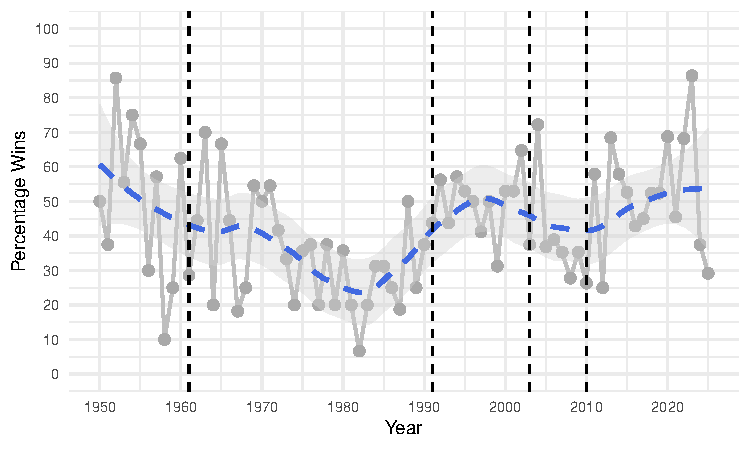
\includegraphics{Formula1_files/figure-latex/unnamed-chunk-90-1} 

}

\caption{Percentage Wins}\label{fig:unnamed-chunk-90}
\end{figure}

We can see that from 1965 and Jim Clark's title, until 2004 and Michael
Schumacher third or fourth title, that is a period of 40 years, no pilot
achieved a win to race ratio over 65\%. And if we filter out the earlier
championships with less than 12 races (where a high percentage is easier
to achieve than when there are more races), the only high percentage
championships are the recent ones, that is after 2000.

The two highest percentages are when Max Verstappen won the title in
2023 with 19 races won over 22, and Alberto Ascari with 6 wins over 7
races. Both achieved more than 85\% win success.

\begin{table}[!h]
\centering\begingroup\fontsize{9}{11}\selectfont

\begin{tabular}{llrrr}
\toprule
year & driverName & nbraces & wins & winspc\\
\midrule
2023 & \includegraphics[width=0.25cm]{/home/runner/work/Formula-1/Formula-1/images/flags/icons8-netherlands-50.png} Max Verstappen & 22 & 19 & 86.4\\
1952 & \includegraphics[width=0.25cm]{/home/runner/work/Formula-1/Formula-1/images/flags/icons8-italy-50.png} Alberto Ascari & 7 & 6 & 85.7\\
1954 & \includegraphics[width=0.25cm]{/home/runner/work/Formula-1/Formula-1/images/flags/icons8-argentina-50.png} Juan Fangio & 8 & 6 & 75.0\\
2004 & \includegraphics[width=0.25cm]{/home/runner/work/Formula-1/Formula-1/images/flags/icons8-germany-50.png} Michael Schumacher & 18 & 13 & 72.2\\
1963 & \includegraphics[width=0.25cm]{/home/runner/work/Formula-1/Formula-1/images/flags/icons8-great-britain-50.png} Jim Clark & 10 & 7 & 70.0\\
2020 & \includegraphics[width=0.25cm]{/home/runner/work/Formula-1/Formula-1/images/flags/icons8-great-britain-50.png} Lewis Hamilton & 16 & 11 & 68.8\\
2013 & \includegraphics[width=0.25cm]{/home/runner/work/Formula-1/Formula-1/images/flags/icons8-germany-50.png} Sebastian Vettel & 19 & 13 & 68.4\\
2022 & \includegraphics[width=0.25cm]{/home/runner/work/Formula-1/Formula-1/images/flags/icons8-netherlands-50.png} Max Verstappen & 22 & 15 & 68.2\\
1955 & \includegraphics[width=0.25cm]{/home/runner/work/Formula-1/Formula-1/images/flags/icons8-argentina-50.png} Juan Fangio & 6 & 4 & 66.7\\
1965 & \includegraphics[width=0.25cm]{/home/runner/work/Formula-1/Formula-1/images/flags/icons8-great-britain-50.png} Jim Clark & 9 & 6 & 66.7\\
\bottomrule
\end{tabular}
\endgroup{}
\end{table}

\newpage

On the other side, it is possible to win the championship by winning
less races. The table below shows the drivers who won the championship
with the lowest win to race ratio :

\begin{table}[!h]
\centering\begingroup\fontsize{9}{11}\selectfont

\begin{tabular}{llrrr}
\toprule
year & driverName & nbraces & wins & winspc\\
\midrule
1964 & \includegraphics[width=0.25cm]{/home/runner/work/Formula-1/Formula-1/images/flags/icons8-great-britain-50.png} John Surtees & 10 & 2 & 20.0\\
1974 & \includegraphics[width=0.25cm]{/home/runner/work/Formula-1/Formula-1/images/flags/icons8-brazil-50.png} Emerson Fittipaldi & 15 & 3 & 20.0\\
1977 & \includegraphics[width=0.25cm]{/home/runner/work/Formula-1/Formula-1/images/flags/icons8-austria-50.png} Niki Lauda & 15 & 3 & 20.0\\
1979 & \includegraphics[width=0.25cm]{/home/runner/work/Formula-1/Formula-1/images/flags/icons8-south-africa-50.png} Jody Scheckter & 15 & 3 & 20.0\\
1981 & \includegraphics[width=0.25cm]{/home/runner/work/Formula-1/Formula-1/images/flags/icons8-brazil-50.png} Nelson Piquet & 15 & 3 & 20.0\\
1983 & \includegraphics[width=0.25cm]{/home/runner/work/Formula-1/Formula-1/images/flags/icons8-brazil-50.png} Nelson Piquet & 15 & 3 & 20.0\\
1987 & \includegraphics[width=0.25cm]{/home/runner/work/Formula-1/Formula-1/images/flags/icons8-brazil-50.png} Nelson Piquet & 16 & 3 & 18.8\\
1967 & \includegraphics[width=0.25cm]{/home/runner/work/Formula-1/Formula-1/images/flags/icons8-new-zealand-50.png} Denny Hulme & 11 & 2 & 18.2\\
1958 & \includegraphics[width=0.25cm]{/home/runner/work/Formula-1/Formula-1/images/flags/icons8-great-britain-50.png} Mike Hawthorn & 10 & 1 & 10.0\\
1982 & \includegraphics[width=0.25cm]{/home/runner/work/Formula-1/Formula-1/images/flags/icons8-finland-50.png} Keke Rosberg & 15 & 1 & 6.7\\
\bottomrule
\end{tabular}
\endgroup{}
\end{table}

We can se that from 1974 until 1987, it was very common to win the world
title with less than 20\% races won. Notably, the Brasilian driver
Nelson Piquet won his 3 world titles by winning less than 20\% of the
races each time.

The record being held by Keke Rosberg who won the 1982 championship by
winning only 1 race out of 15.

Note tat in 2025 the win to races ratio was one of the lowest in the
recent years : with only 29\% wins, Lando Norris was able to win the
title, even with less victories (7) than Verstappen (8). His teammate
Piastri was able to win the same number of races.

\newpage

\subsubsection{4.3.2 Points and Rules}\label{points-and-rules}

The evolution of points systems and rules in Formula 1 has undergone
significant changes over the years, reflecting the sport's adaptability
to enhance competition and viewer engagement. Understanding these
modifications is crucial for properly interpreting statistics and
achievements across different eras of racing.

One of the most notable changes in the points system involves the method
of calculating scores based on race results. In earlier years, drivers
earned points for finishing in the top positions, but not all results
were counted towards the championship. For instance, the introduction of
the ``\textbf{8 best results}'' system allowed drivers to select their
top performances to be counted toward their final tally. This change
meant that a driver could have an off day in a few races but still
remain competitive based on their standout performances. The revised
approach promotes consistency and allows for some leeway, encouraging
drivers to focus on achieving high results in selected races rather than
simply accumulating points in every competition.

In recent years, the integration of new formats such as \textbf{sprint
races} has further influenced the dynamics of scoring. Sprint events,
which typically take place on weekends with traditional Grand Prix
races, offer additional points opportunities. This development adds an
exciting layer to the race weekend, allowing drivers to earn points not
just through their main races but also by performing well in shorter
sprints. The introduction of these sprints has reshaped strategies,
pushing teams to adapt their approaches to maximize potential points
across various race formats.

Another element that has gained attention is the inclusion of points
awarded for the \textbf{fastest lap} during a race, further enriching
the competitive landscape. By recognizing drivers who secure the fastest
lap, this rule incentivizes aggressive racing strategies, compelling
drivers to push their limits even when their overall position may not
warrant it. This addition exemplifies how changes in rules can elevate
the excitement and intensity of each race.

As we compare drivers and their results over time, it is important to
note that we will not consider sprint races or fastest laps in our
study. Our analysis will focus solely on race results, and we will take
into account all points awarded across each driver's career. This
approach allows us to maintain a more consistent basis for comparison,
ensuring that our findings reflect the fundamental aspects of
performance in Formula 1.

The implications of these transformed points systems extend beyond mere
statistics. They affect team and driver strategies, influencing how
races are approached. Teams may prioritize specific races or adopt
riskier tactics, knowing that achieving the fastest lap or excelling in
a sprint can contribute critically to their overall standings. This
fosters a more vibrant competitive environment where drivers constantly
seek opportunities to maximize their returns, complicating the notion of
what it means to be successful in Formula 1.

Moreover, when comparing drivers across different eras, it becomes
essential to contextualize their accomplishments within the frameworks
established by the rules at the time. Historical figures like Juan
Manuel Fangio, for example, achieved remarkable titles under a vastly
different scoring system, contrasting sharply with the multifaceted
approach seen today. Understanding these differences in rules and points
systems allows fans and analysts to appreciate the evolution of the
sport while acknowledging the unique challenges faced by drivers across
generations.

\newpage

The plot below shows the number of points given according to the race
final position :

\begin{figure}

{\centering 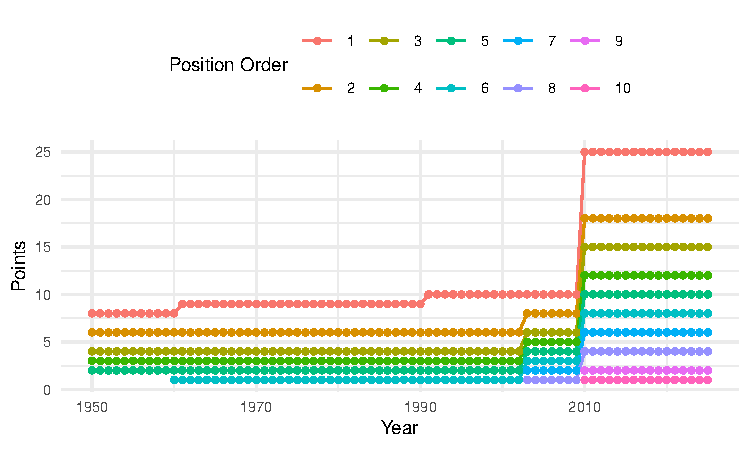
\includegraphics{Formula1_files/figure-latex/unnamed-chunk-93-1} 

}

\caption{Points per Year}\label{fig:unnamed-chunk-93}
\end{figure}

Until 1959, the scoring system for races awarded the winner 8 points,
with an additional point granted for the fastest lap achieved during the
race. However, in 1960, the point for the fastest lap was eliminated,
and instead, the driver finishing in 6th position would receive one
point. The following year, in 1961, the points awarded to the winner
increased to 9, further evolving the scoring structure. By 1991, winners
would receive 10 points, while other position points remained unchanged.
The scoring system underwent a significant revision in 2003, when
drivers other than the winner began to receive an additional 2 points.
Additionally, drivers finishing in 7th and 8th positions would earn 2
points and 1 point, respectively. By 2010, the rules changed again,
increasing the winner's points to 25 and extending points to the top 10
finishers.

Although not depicted in this analysis, it's worth noting that in 2019,
a point for the fastest lap was reintroduced. Furthermore, between 1950
and 1990, only certain race results contributed towards the championship
standings, indicating fluctuations in how scoring impacted overall
competitive success during that period.

\newpage

The plot below shows the percentage difference :

\begin{figure}

{\centering 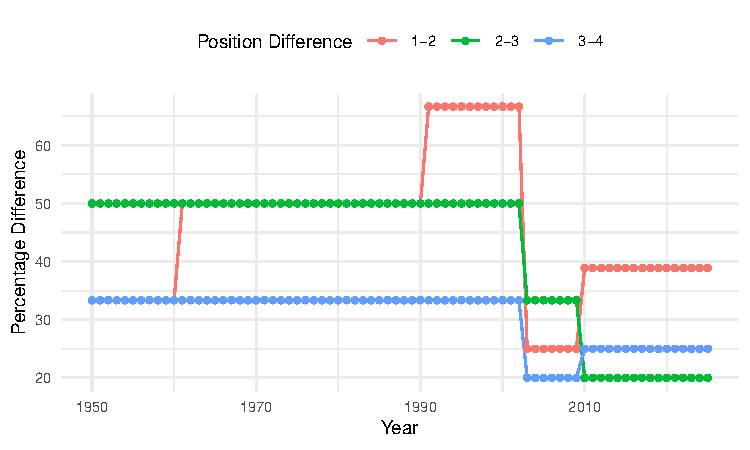
\includegraphics{Formula1_files/figure-latex/unnamed-chunk-94-1} 

}

\caption{Percentage Difference}\label{fig:unnamed-chunk-94}
\end{figure}

From 1950 until 1959, the winner received 33\% more points than the
second-place driver, who was awarded 50\% more points than the driver
finishing in third, while the third place earned 33\% more points than
the fourth. However, in 1960, the rules shifted so that the winner
received 50\% more points than the second-place driver, and this
percentage increased to 66\% in 1991. Starting in 2003, this difference
in points began to decrease significantly, with a slight increase in
2010, resulting in the winner obtaining approximately 40\% more points
than the second-place finisher, who in turn received 20\% more than the
third, while the third place earned 25\% more than the fourth.

This plot illustrates how the importance of finishing position has
diminished since 2003, suggesting that the risks associated with
overtaking another driver may no longer justify the potential rewards.
As drivers weigh the dangers of overtaking, the incentive structure of
points allocation reflects a changing competitive landscape, where
maintaining position may become a more strategic choice.

\newpage

The table below displays championships in which the driver who earned
the highest total points did not win the title. This occurred because
only a portion of these points were counted, allowing the second-place
driver to secure the championship with a greater proportion of their
retained points :

\begin{table}[!h]
\centering\begingroup\fontsize{9}{11}\selectfont

\begin{tabular}{lllll}
\toprule
year & driverNameChampion & pointsChampion & driverNameBest & pointsBest\\
\midrule
1964 & \includegraphics[width=0.25cm]{/home/runner/work/Formula-1/Formula-1/images/flags/icons8-great-britain-50.png} John Surtees & 40(40) & \includegraphics[width=0.25cm]{/home/runner/work/Formula-1/Formula-1/images/flags/icons8-great-britain-50.png} Graham Hill & 41(39)\\
1988 & \includegraphics[width=0.25cm]{/home/runner/work/Formula-1/Formula-1/images/flags/icons8-brazil-50.png} Ayrton Senna & 94(90) & \includegraphics[width=0.25cm]{/home/runner/work/Formula-1/Formula-1/images/flags/icons8-france-50.png} Alain Prost & 105(87)\\
\bottomrule
\end{tabular}
\endgroup{}
\end{table}

In the world of Formula 1 racing, championship titles are not solely
determined by the total points a driver accumulates over the season.
This nuance became particularly evident in dramatic cases such as those
of John Surtees in 1964 and Ayrton Senna in 1988.

In 1964, John Surtees clinched the World Championship with a total of 40
points, and importantly, all of these points were eligible for inclusion
in the championship standings. Surtees faced stiff competition from his
rival, Graham Hill, who ended the season with 41 points---just a single
point ahead. However, not all of Hill's points were counted towards the
championship, as only 39 points were eligible, thus causing him to lose
the title to Surtees. This incident serves as a poignant reminder of the
impact of point retention rules in determining the final standings,
which can overshadow pure performance metrics.

Fast forward to 1988, when the same theme of point retention played out
yet again in a fierce rivalry between Ayrton Senna and Alain Prost.
Senna finished the season with an impressive 94 points, out of which 90
points were counted towards his championship total. Conversely, Alain
Prost amassed a remarkable 105 points but faced a significant setback as
only 87 of these points were deemed eligible for the championship
classification. This discrepancy ultimately placed Prost in second
position, despite his overall higher point total.

\newpage

The plot below shows the total number of points given per year :

\begin{figure}

{\centering 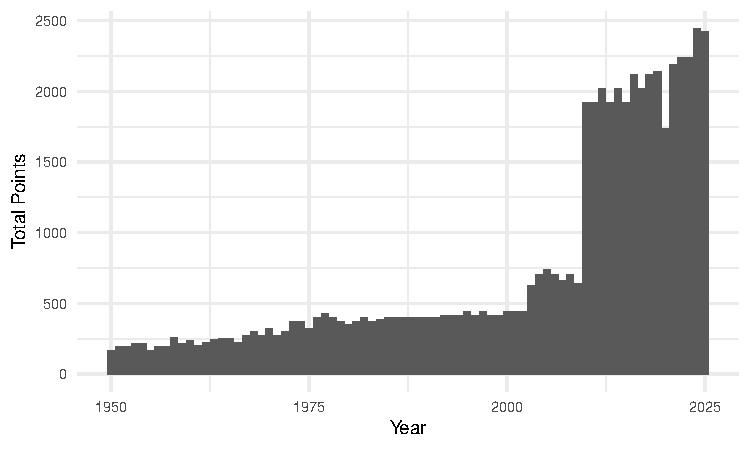
\includegraphics{Formula1_files/figure-latex/unnamed-chunk-96-1} 

}

\caption{Total Points per Year}\label{fig:unnamed-chunk-96}
\end{figure}

In conclusion, the changes in points and rules over time significantly
impact how success and performance are measured in Formula 1. The
transition from early systems to contemporary practices reflects the
sport's commitment to enhancing competitiveness and excitement.
Analyzing these developments provides crucial context for assessing
driver achievements and understanding the strategic decisions made by
teams and drivers alike. The interplay between points systems, race
formats, and performance metrics illustrates the complexity of the sport
and highlights how Formula 1 continually evolves to captivate its
audience.

\newpage

\subsubsection{4.3.3 Comparing Across Eras}\label{comparing-across-eras}

The previous two sections of this chapter have each peeled back one
layer between a driver's statistics and his ability: the car he drove,
and now the framework in which he raced. Putting the framework's
dimensions together, the drift across the championship's history is
stark. In 1950 a title was decided over 7 races; by the 2020s, a season
comprises roughly four times as many, multiplying the occasions on which
a strong driver can win and score. The points attached to a victory have
grown from 8 to 25, and the widening of the points-paying positions ---
from the top five to the top ten --- further rewards consistency over
the long calendars of the modern era. And careers themselves have
stretched: where drivers of the 1950s typically raced fewer than ten
seasons, the front-runners of today contest twenty or more, giving each
generation more seasons in which to stack titles.

None of this is evidence that modern drivers are superior; it is
evidence that the units in which their records are denominated have
inflated. A win in 1953 was scarcer by a factor of three than a win in
2023, a title cost fewer conversions, and a season offered fewer
opportunities to convert them at all. Raw tallies --- the 105 titles,
wins and points enumerated at the opening of this chapter --- therefore
measure opportunities converted, not skill displayed.

The conclusion for the remainder of this study follows directly. To
compare drivers of different eras fairly, the framework must be held
constant along all three dimensions:

\begin{itemize}
\tightlist
\item
  \textbf{Scoring} --- each result should be awarded the same points
  regardless of the season in which it was achieved, normalizing away
  the evolution from the 8-point systems of the 1950s to the 25-point
  system in force today;
\item
  \textbf{Calendar} --- each season should be reduced to a common number
  of races, so that a champion of a 7-round calendar is not penalized
  relative to a champion of a 24-round one;
\item
  \textbf{Longevity} --- each career should be measured over the same
  number of seasons, since the inflation of career length across the
  decades mechanically favours recent drivers in any cumulative
  statistic.
\end{itemize}

Only under these three normalizations do titles, wins and points become
comparable quantities --- and only then can the question left open in
Section 4.1.6, whether Fangio would have matched today's champions on
equal terms, be answered with data rather than opinion. Chapter 5
implements exactly these transformations.

\newpage

\section{9. References}\label{references}

{[}1{]} Hergé. 1956. ``The Calculus Affair''
\url{https://www.tintin.com/en/albums/the-calculus-affair}

\vspace{10pt}

{[}1{]} Jean-Luc. 2019. ``Tintin -- The Calculus Affair -- The liberties
of English translation''
\url{https://tintinomania.com/tintin-affaire-tournesol-anglais-brabham}

\vspace{10pt}

{[}2{]} Kaggle ``Formula 1 World Championship (1950 - 2024)''
\url{https://www.kaggle.com/datasets/rohanrao/formula-1-world-championship-1950-2020}

\vspace{10pt}

{[}3{]} Tracing Insights ``Race Data''
\url{https://github.com/TracingInsights/RaceData}

\vspace{10pt}

{[}4{]} Dataset copied to GitHub. Available at:
\url{https://github.com/jmr-lab/Formula-1} (Accessed: 2026).

\vspace{10pt}

{[}5{]} Flags from icons8 :
\url{https://icons8.com/icons/set/flags--style-color}

\vspace{10pt}

{[}3{]} Rafael Irizarry. ``Introduction to Data Science.''
\url{https://rafalab.dfci.harvard.edu/dsbook/}

\vspace{10pt}

{[}8{]} Cover image from SVG SILH
\url{https://svgsilh.com/c3c3c3/image/309862.html}

\vspace{10pt}

{[}9{]} Icons from Font Awesome \url{https://fontawesome.com/}

\vspace{10pt}

{[}10{]} The text of this report was reviewed by DuckAI, an AI language
model that also assisted in reviewing and correcting some of my code :
\url{https://duck.ai/}

\end{document}
